% !Mode:: "TeX:UTF-8"
%!TEX program  = xelatex
% ============================================================
% 华为杯（中国研究生数学建模竞赛）论文主稿
% 版式由 gmcmthesis.cls 提供，本文件负责内容组织与门禁标签。
% 编译方式：XeLaTeX
% ============================================================
\documentclass[bwprint]{gmcmthesis}

\hypersetup{hidelinks, allcolors=black}

\usepackage{subfig}
\usepackage{siunitx}
\usepackage{graphicx}
\usepackage{placeins}

% 图/表全篇连续编号
\counterwithout{figure}{section}
\counterwithout{table}{section}

% 图件目录：各问图件与手绘图
\graphicspath{{figures/}{../Q1/figures/}{../Q2/figures/}{../Q3/figures/}{../灵敏度分析/figures/}{../手绘图/}}

% 算法
\usepackage[noend]{algpseudocode}
\usepackage{algorithmicx,algorithm}
\floatname{algorithm}{算法}
\renewcommand{\algorithmicrequire}{\textbf{输入:}}
\renewcommand{\algorithmicensure}{\textbf{输出:}}

% 引用以上标数字角标显示
\makeatletter
\def\@cite#1#2{\textsuperscript{[{#1\if@tempswa , #2\fi}]}}
\makeatother

%===================== 建模论文题目与封面信息 =====================

\title{服务于脑机接口与精神性疾病诊断的脑电图计算模型}
\baominghao{\hspace{6em} 20260900001}
\schoolname{\hspace{5.8em} 参赛学校}
\membera{\hspace{6em} 队员甲}
\memberb{\hspace{6em} 队员乙}
\memberc{\hspace{6em} 队员丙}

%=======================================================

\begin{document}
\label{body:start}

\maketitle

% ============================================================
% 摘要与关键词
% ============================================================
\begin{abstract}\label{abstract:start}
脑电驱动的计算模型是连接神经机制研究与临床应用的桥梁。本文围绕视觉认知实验的三导联脑电记录，建立资料预处理、多尺度前向计算模型与认知宏观模型的完整链路，并用四份赛题记录完成定量分析。

\textbf{针对问题一}，本文以伪迹抑制率与视物特征保留度双准则比较了七类降噪方案。实测显示三导联脑电与心电模板的最大相关度仅 0.35 至 0.45，心电伪迹并不显著；而 0.5 至 30 Hz 带通把左右可分性压低到 0.412 至 0.579，在两个项目二记录上低于随机水平。据此本文提出\textbf{窄目标化的稳健软截断方案}，只压缩超出 10 倍稳健尺度的极端采样点，不做高通或带通。该方案把 99 分位单试次峰值压低 \textbf{0.325}，把左右可分性提高到 \textbf{0.5525}，相对带通方案提高 0.0592，配对检验 $t$ 值 4.461、$p$ 值小于 0.001，相对原始信号提高 0.0071。逐点单样本 $t$ 检验配合错误发现率控制显示两个项目二记录有 71 至 205 个显著时间点，两个项目一记录没有显著时间点。三高斯分量拟合在项目二记录上的决定系数达 0.972 至 0.991。

\textbf{针对问题二}，本文建立五级串联的\textbf{多尺度前向计算模型}，依次为 LGN 时空滤波、形状选择与除法归一化、Wilson--Cowan 介观集群、Kuramoto 宏观同步与序参数、头皮导联场观测。模型的镜像性误差为 0.0000，预测左右刺激的偏侧响应符号相反、Fz 对镜像差异不敏感，与实测一致。模型预测的偏侧时程与实测相关系数达 \textbf{0.8718}。由机制导出的\textbf{形状—空间联合特征}在四份记录上的交叉验证 AUC 为 0.5250 至 0.5792，早期形状特征与晚期偏侧特征的贡献量级相当。

\textbf{针对问题三}，本文建立\textbf{双源延迟耦合认知宏观模型}，视觉通路 120 个振子、海马体通路 80 个振子，记忆通路经延迟与增益耦合到视觉通路，前额叶整合变量含符合项。辨识得到记忆通路延迟 \textbf{0.271 s}、增益 \textbf{5.310}、整合时间常数 0.570 s，加权残差平方和为 0.0245。模型在两个项目二记录上的相关系数为 \textbf{0.9256} 与 \textbf{0.9305}，归一化均方根误差为 0.14 至 0.17；在两个项目一记录上拟合失败，与其视觉响应没有显著时间点的事实一致。敏感性分析显示两路权重的可辨识性比延迟与增益高一个数量级。

本文的核心发现是：承载视物信息的低频慢电位与设备滤波器所去除的成分是同一成分，因此去噪必须窄目标化；左右差异来自镜像的皮层空间分布；认知过程需要双源结构，记忆来源不可缺失。

\keywords{脑电计算模型\quad 窄目标化去噪\quad 多尺度前向模型\quad 左右区分特征\quad 双源认知模型}\label{abstract:end}

\end{abstract}

\pagestyle{plain}

\maketoc
\clearpage

% ============================================================
% 正文
% ============================================================

\section{问题重述}

\subsection{问题背景}

大脑活动可由侵入性与非侵入性两类神经影像方法记录，皮层脑电图与脑电图分别是两类技术的代表。侵入性技术受手术风险与信号随时间退化的限制，非侵入性脑电图因此在探索人类大脑活动方面具备更广的应用前景。脑电驱动的计算模型是连接基础神经科学研究与神经临床应用的核心桥梁，它既能为脑机接口的脑活动解码与交互控制提供算法框架，也能在神经机制探索与神经性疾病临床研究中承担虚拟实验平台的功能，通过仿真完成实验方案预演与科学假设的定量检验。

运动皮层产生的脑电 $\beta$ 节律在自主运动期间受到抑制，运动结束后幅度短暂回升，两者合称 $\beta$ 波段调制。精神分裂症患者的运动后 $\beta$ 反弹显著减弱，且其幅度与症状严重程度相关。阿尔茨海默症患者早期常出现明显记忆减退，现有量表诊断不够严谨，而源于海马体的信号逐渐迟缓且微弱可能是更早的指标。这些临床线索都指向同一个技术需求：把微观神经元活动规律、大脑神经网络与电生理特点结合起来的脑电计算模型。

从空间尺度看，脑电计算模型分三个层次。微观尺度以 Hodgkin--Huxley 模型与耦合漏电积分发放神经元为代表，描述单个细胞或微电路；介观尺度以 Wilson--Cowan 神经集群模型为代表，用平均场方程描述兴奋性与抑制性神经元群的平均活动；宏观尺度以 Kuramoto 模型为代表，用相位耦合描述大量弱耦合振子的同步行为，并可由脑网络结构连接矩阵把多个局部模型耦合起来。脑电本身是对大量神经元同步现象序参数的一种观测。

把三个尺度接起来并不容易。宏观模型引入的序参数可以反映同步后的脑电信号，却没有考虑神经元的空间分布，而不同分布给出的序参数并不相同。刺激引起的皮层响应又无法直接观测神经元的空间分布。把该问题转化为数学反问题会遭遇非唯一性与传输复杂性，实际应用价值有限。本文需要建立视觉刺激物形状与皮层响应神经元分布之间的联系，以及脑电观测与皮层响应神经元之间的联系。

\FloatBarrier
\begin{figure}[htp!]
\centering

\includegraphics[width=0.68\textwidth]{fig_roadmap.pdf}
\caption{全文技术路线图。左侧为数据解析、去噪与响应提取，右侧为多尺度建模与认知分析。}
\label{fig:roadmap}
\end{figure}
\FloatBarrier

图 \ref{fig:roadmap} 给出全文的技术路线。数据侧从四份原始记录出发，经事件解析、窄目标化去噪与响应提取得到干净分段与响应特征；模型侧由多尺度前向计算模型给出左右区分特征，再扩展为双源认知宏观模型并完成参数辨识与分层分析。两侧通过问题一的派生数据衔接。

\subsection{问题提出}

题面给出的视觉认知实验在 F3、Fz、F4 三个前额点位采集脑电，针对两个识别项目。项目一在目标出现之前已知目标位置，只等待其出现；项目二在目标出现之前不知道目标位置，只知道目标形状。四份记录采样率为 256 Hz，每份 10 个通道、各含 100 个试次。通道语义为 Fz、F3、F4 原始信号，FzDecon、F3Decon、F4Decon 设备自带滤波输出，ECG 参考，VisCue 视觉提示，TgtAct 目标应答，TimeStamp 时间戳。题面要求避免直接使用设备自带滤波通道。

\FloatBarrier
\begin{figure}[htp!]
\centering
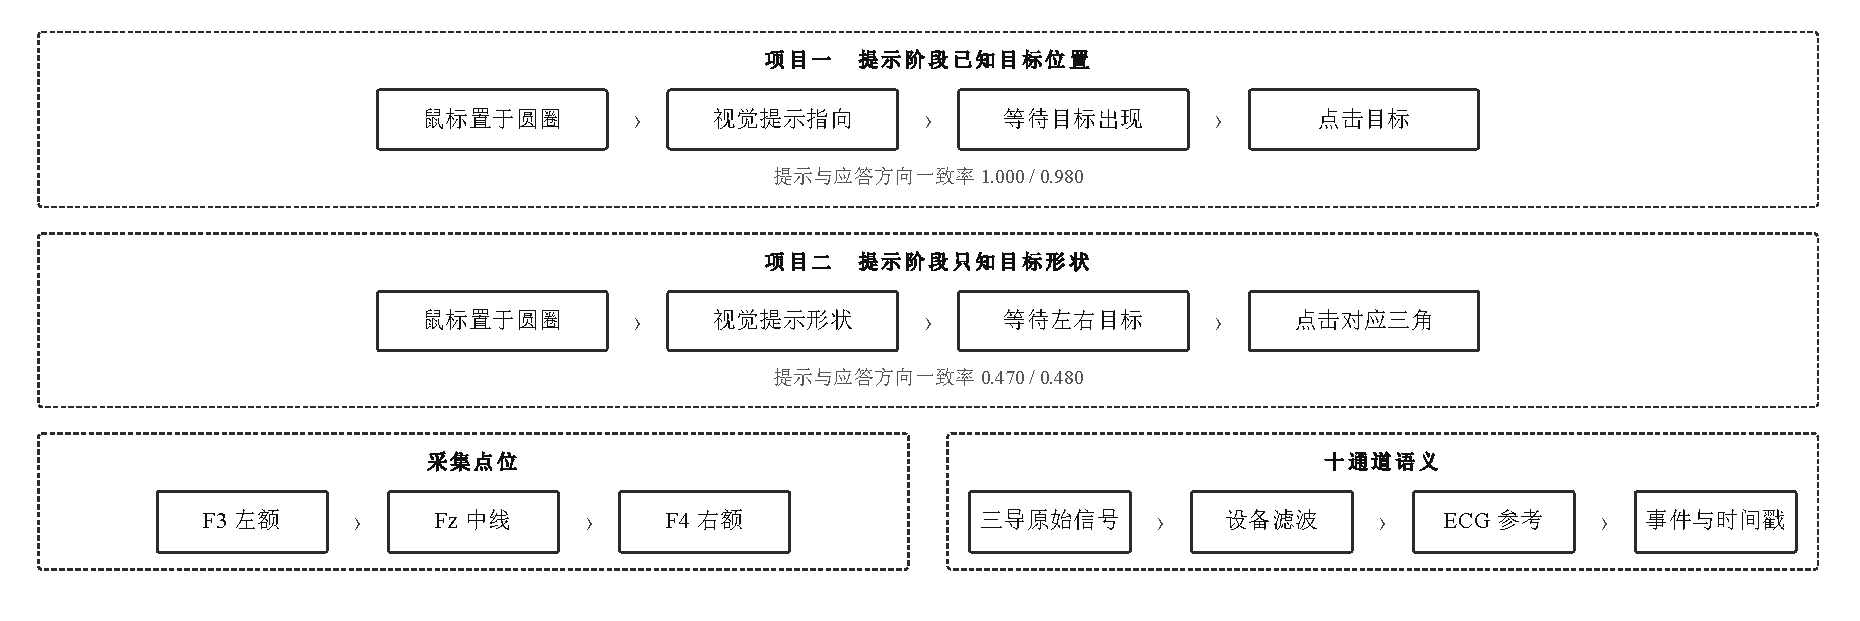
\includegraphics[width=0.98\textwidth]{fig_experiment_design.pdf}
\caption{实验设计与数据结构。上行为项目一与项目二的时序对比，下行为三导采集点位与十通道语义分组。}
\label{fig:design}
\end{figure}
\FloatBarrier

图 \ref{fig:design} 对比了两个项目的时序。项目一在提示阶段即给出目标位置，因此提示方向与应答方向一致率接近 1；项目二只给出形状，位置在提示后约 2 s 才出现，因此一致率接近随机水平。这一结构差异是理解全部数据结果的前提。

视觉刺激产生 P300 现象，即大脑在接收特定视觉任务刺激后约 250 至 500 ms 内在中央—顶区产生的一个正向事件相关电位。由于存在各种噪声，原始脑电不能直接显示 P300 波形。据此提出三项建模任务。

\begin{enumerate}
\item 针对实验项目一与实验项目二，对给定脑电数据做资料预处理，在保留视物形状脑电特征的前提下去除运动、眨眼等伪影，提取不同观测点位的有效视觉响应并拟合相应曲线。
\item 建立脑电计算模型，说明从 LGN 到皮层、再到头皮观测脑电的机理；解释左右三角刺激产生脑电信号差异的形成机制；给出能区分左右三角形视觉刺激响应的特征表示。
\item 截取与视觉认知相关联的信号，其终点取应答响应之前约 100 ms；借助第二项任务建立的脑电信号形成机制，并考虑信号可能同时来源于海马体与 LGN 等，建立认知的宏观模型，并用题目提供的脑电信号分析该模型。
\end{enumerate}

\FloatBarrier
\begin{figure}[htp!]
\centering
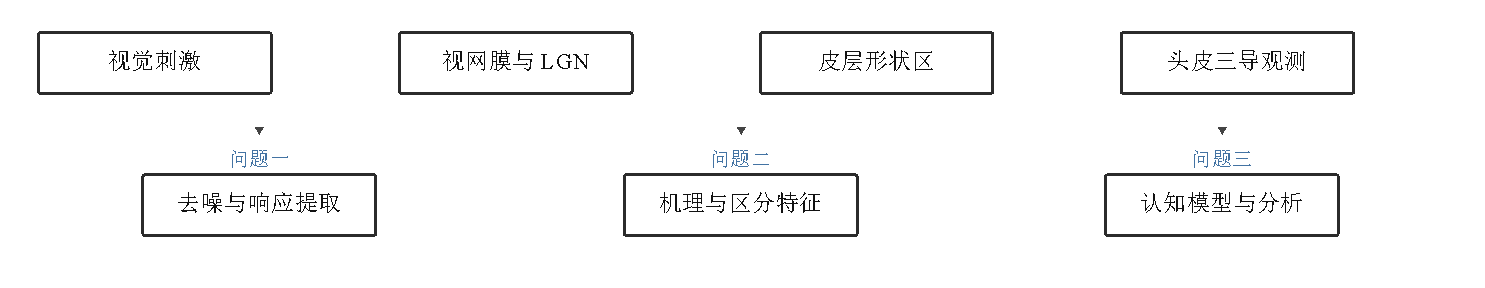
\includegraphics[width=0.98\textwidth]{fig_problem_analysis.pdf}
\caption{问题分析流程图。上半部分为视觉通路的前向链，下半部分为三项建模任务的任务边界。}
\label{fig:problem}
\end{figure}
\FloatBarrier

图 \ref{fig:problem} 把三项任务放在同一条通路上定位。问题一处理从原始记录到有效响应的数据侧问题，问题二处理从 LGN 到头皮观测的机理侧问题，问题三在机理之上增加记忆通路并做参数辨识。三项任务共享同一套分段信号与同一套观测算子。

题面提示，神经生理学证据表明人脸等物体的识别通过检测特定空间方式排列的某些特征实现。成年猴子的单细胞记录显示，颞下皮层的一个神经元对具象面部与仅由圆圈、水平条和一对水平斑点构成的简化图标产生相似反应，一旦轮廓、双眼与嘴部的相对结构缺失，响应几乎可忽略。这一证据说明形状识别的计算基础是特征组合的匹配，而不是像素级比对，本文的问题二模型据此设计。

题面还提示应答不一定正确，也可能没有及时应答。这要求认知模型把认知过程与应答行为分开刻画，不能假设应答方向等于提示方向。本文在问题三中对这一点做了显式的分层分析。

\section{模型假设与符号说明}

\subsection{模型假设}

本文全部假设均与题面、数据特征和模型需求对应，逐条列出。

\begin{enumerate}
\item 刺激后 0 至 1000 ms 窗口内的脑电可分解为任务锁定成分、背景自发振荡与非神经伪影三部分，三者在叠加意义上近似可分。该假设使分段后的逐试次信号可以用线性算子处理。
\item 心电伪迹在各试次中波形一致、仅增益不同，因此可由 ECG 通道对齐后的中位模板刻画。本文用实测相关度检查该假设是否成立，而不是默认成立。
\item 运动与电极瞬变在时域表现为远高于背景的稀疏极端偏移，可由稳健尺度界定。该假设使软截断只作用于少量采样点。
\item 低频慢电位属于任务相关信息，不是伪影。该假设由实测判别性能支持，详见问题一。
\item 刺激前 0.2 s 窗口内不含任务相关成分，可作基线。两个项目一记录的提示与应答一致率接近 1，说明提示前被试处于等待状态。
\item 视觉通路可用视网膜、LGN、初级视皮层、高级形状区、头皮的串行前向链刻画，各阶段时空尺度依次增大。该假设使五级模型可逐级串联。
\item LGN 的时空响应可分离为空间差分高斯核与因果 Gamma 时间核的乘积。差分高斯给出中心—周边拮抗的对比敏感特性，因果 Gamma 核给出延迟与瞬态响应。
\item 形状选择性神经元对特定空间排列的特征组合响应，其偏好模板在左右刺激之间互为镜像。该假设是左右差异的几何来源。
\item 皮层神经元群的平均活动可由 Wilson--Cowan 型平均场方程描述，兴奋与抑制耦合强度在刺激期间近似恒定。
\item 头皮电位是大量神经元群同步活动的宏观汇集，观测对象是序参数包络本身。该假设直接来自题面对序参数的说明。
\item 前额三导 Fz、F3、F4 的导联场随源到电极距离单调衰减，构成一个空间低通算子。
\item 认知过程由两条通路共同承担，LGN 与皮层通路提供直接视觉信息，海马体与前额通路提供记忆对照信息。该假设对应题面关于信号可能同时来源于海马体与 LGN 的提示。
\item 海马体通路相对视觉通路存在传导延迟与增益，且其群体活动的包络比视觉通路更慢。慢化假设使增益在形状拟合中可辨识。
\item 前额叶认知区对两路信息做一致性整合，整合变量含符合项，只在两路信息时间对齐时给出额外增益。
\item 应答方向与提示方向可以不一致，认知过程与应答行为分开刻画。
\end{enumerate}

\subsection{符号说明}

下表列出全文符号的口径。符号按层次分组，上标或下标用于区分通道、条件与通路，未在下表出现的局部符号在其首次使用时就地说明。

% 符号表使用非浮动 longtable 容器：符号内容实际超过一页，自动跨页并重复表头；
% 进入前保存 table 计数、结束后恢复，保证符号表不占用正式结果表编号。
\renewcommand\arraystretch{1.15}
\newcolumntype{L}{>{\quad}X}
\newcolumntype{P}[1]{>{\centering\arraybackslash}p{#1}}
\newcounter{huaweisymbolsavetable}
\setcounter{huaweisymbolsavetable}{\value{table}}
\noindent\begin{longtable}{|P{2.6cm}|>{\raggedright\arraybackslash}p{\dimexpr0.92\textwidth-2.6cm-4\tabcolsep-3\arrayrulewidth\relax}|}
  \hline
  符号    &   \quad 意义 \\
  \hline
  \endfirsthead
  \hline
  符号    &   \quad 意义（续） \\
  \hline
  \endhead
  $c$ & 观测导联，取 $c \in \{\mathrm{Fz},\mathrm{F3},\mathrm{F4}\}$ \\
  $x_c(t)$ & 导联 $c$ 的连续记录信号，单位 $\si{\micro\volt}$ \\
  $e_c^{(i)}(t)$ & 第 $i$ 个试次、导联 $c$ 的分段信号，窗口取刺激前 $0.2$ s 至刺激后 $1.0$ s \\
  $b_c^{(i)}$ & 第 $i$ 个试次的基线值，取刺激前窗口均值 \\
  $\sigma_c$ & 导联 $c$ 的稳健尺度，取 $1.4826$ 倍中位绝对偏差 \\
  $T_c(\tau)$ & 导联 $c$ 的心电伪迹中位模板 \\
  $g_i$ & 第 $i$ 个试次的心电模板增益 \\
  $\rho_i$ & 第 $i$ 个试次分段与心电模板的相关系数 \\
  $z_0, z_1$ & 心电条件阈值与软截断阈值，分别取 $6$ 与 $10$ \\
  $A_c, \lambda_c$ & 导联 $c$ 的响应峰值幅值与潜伏期 \\
  $\Lambda_c$ & 导联 $c$ 的偏侧指数 \\
  $p_c(t)$ & 导联 $c$ 在时刻 $t$ 的逐点检验 $p$ 值 \\
  $I(\mathbf{x},t)$ & 视网膜输入强度分布 \\
  $L(\mathbf{x},t)$ & LGN 输出场 \\
  $K_{\mathrm{LGN}}$ & LGN 时空响应核 \\
  $\sigma_c, \sigma_s$ & 差分高斯的中心与周边尺度 \\
  $\tau_L$ & LGN 因果 Gamma 时间核的时间常数 \\
  $\mathbf{w}_j(\mathbf{x})$ & 第 $j$ 个皮层单元的偏好特征模板 \\
  $z_j(t), u_j(t)$ & 第 $j$ 个皮层单元的匹配能量与归一化驱动 \\
  $E_j(t), I_j(t)$ & 第 $j$ 个集群的兴奋与抑制平均活动 \\
  $w_{EE}, w_{EI}, w_{IE}, w_{II}$ & 集群内自兴奋、自抑制与群间耦合强度 \\
  $\tau_E, \tau_I$ & 兴奋与抑制活动的时间常数 \\
  $\theta_n(t), \omega_n$ & 第 $n$ 个振子的相位与固有频率 \\
  $C_{np}, \tau_{np}$ & 结构连接权重与传导延迟 \\
  $K$ & 全局耦合缩放参数 \\
  $r(t), \psi(t)$ & Kuramoto 序参数幅值与平均相位 \\
  $A_{mn}$ & 第 $n$ 个源到第 $m$ 个电极的导联场权重 \\
  $y_m(t)$ & 第 $m$ 个电极的头皮观测或预测信号 \\
  $f_{\mathrm{shape}}$ & 形状编码特征量，早期窗中线导联的平均幅值 \\
  $f_{\mathrm{space}}$ & 空间偏侧特征量，晚期窗偏侧两导的幅值差 \\
  $\mathbf{z}, \delta$ & 联合特征向量与线性判别判据值 \\
  $\theta_n^{V}, \theta_n^{H}$ & 视觉通路与海马体通路的振子相位 \\
  $\omega_V, \omega_H$ & 两通路的固有频率 \\
  $K_{VV}, K_{HH}, K_{VH}, K_{HV}$ & 通路内与通路间耦合强度 \\
  $\tau_H, g_H$ & 海马体通路传导延迟与增益 \\
  $\tau_H^{\mathrm{slow}}$ & 海马体通路包络的慢化时间常数 \\
  $r_V(t), r_H(t)$ & 两通路的序参数 \\
  $R(t)$ & 前额叶认知整合状态量 \\
  $\beta_V, \beta_H, \gamma$ & 视觉权重、记忆权重与符合项系数 \\
  $\tau_R$ & 认知整合时间常数 \\
  $\Phi$ & 记忆回路维持强度量 \\
  $W_C$ & 认知信号截取窗口，终点取应答前约 $100$ ms \\
  \hline
\end{longtable}
\setcounter{table}{\value{huaweisymbolsavetable}}

\section{问题一模型建立与求解}

\subsection{问题分析与模型建立}

本问的任务目标是把原始脑电转化为可比较的有效视觉响应。任务的难点不在去噪本身，而在去噪与特征保留之间的取舍：题面明确指出，现有多种处理方案虽然能去除伪影，但同时也破坏了反映视物的脑电特征。因此本问必须先把去噪目标形式化，再据此选择算子。

\FloatBarrier
\begin{figure}[htp!]
\centering
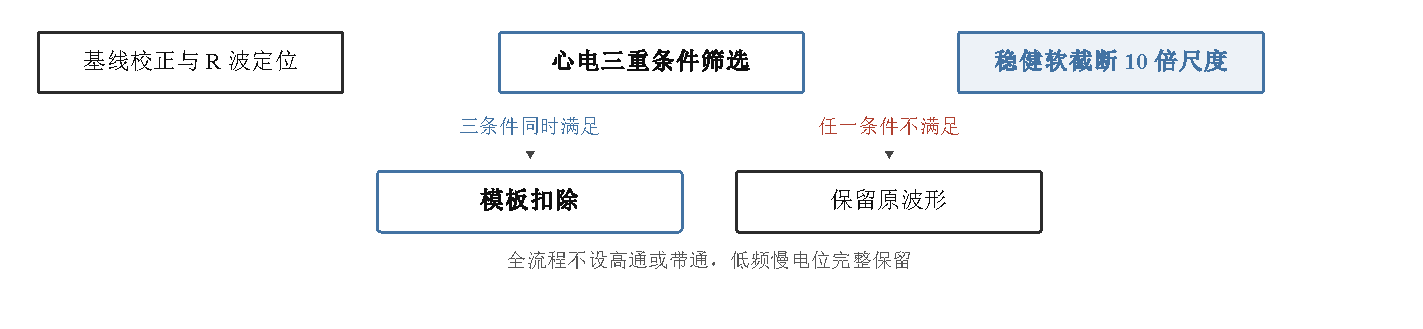
\includegraphics[width=0.98\textwidth]{fig_q1_denoise_flow.pdf}
\caption{窄目标化去噪流程。条件不满足时保留原波形，只有三重条件同时成立才执行模板扣除。}
\label{fig:q1flow}
\end{figure}
\FloatBarrier

图 \ref{fig:q1flow} 给出本文去噪流程。流程的关键在于条件筛选环节：模板扣除必须同时通过相关度、幅度与增益三重条件，任一条件不成立就跳过；软截断只压缩极端采样点；全流程不设高通或带通环节。

\subsubsection{数据条件与分段定义}

四份记录合计 $905337$ 个采样点、$400$ 个试次、总时长约 $3536.5$ s。探索性分析显示四份记录均无缺失值、无重复时间戳，时间戳步长恒为 $1/256$ s。F3 与 F4 通道存在达到设备量程的饱和采样点，四份记录合计约 $3.4$ 万个。三导联标准差为 $53$ 至 $325$ $\si{\micro\volt}$，而稳健尺度仅 $28$ 至 $191$ $\si{\micro\volt}$，峰度最高达 $5.82$，呈显著重尾分布，说明少数高幅试次主导了方差。以 $6$ 倍稳健尺度为界，逐导联伪迹试次比例为 $0.11$ 至 $0.33$，四份记录平均 $0.228$。

\FloatBarrier
\begin{figure}[htp!]
\centering
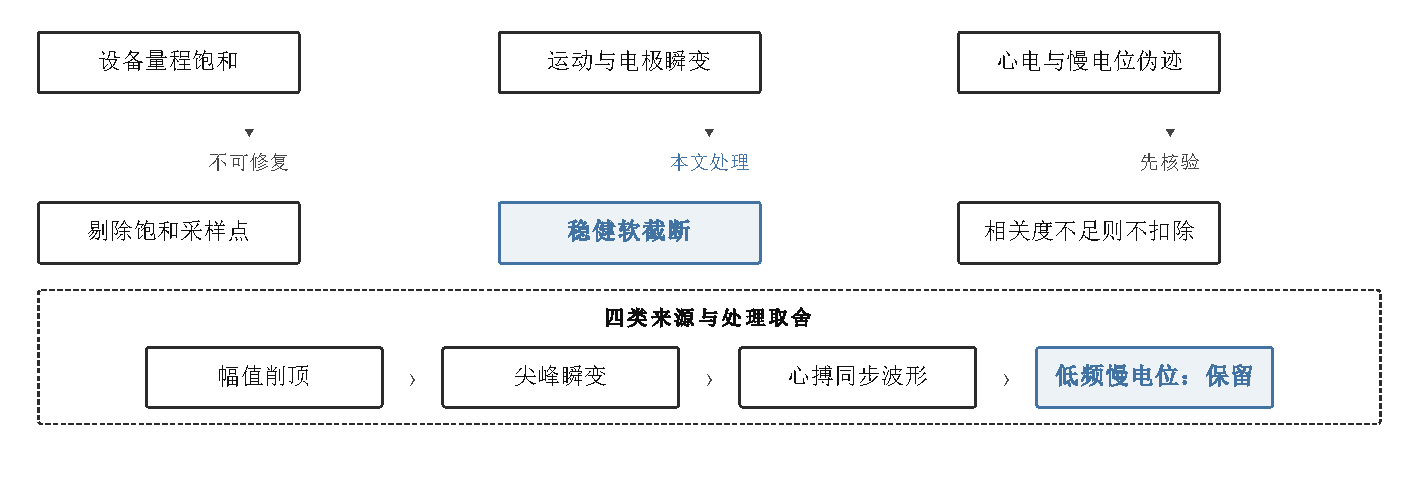
\includegraphics[width=0.98\textwidth]{fig_artifact_sources.pdf}
\caption{数据质量与伪迹来源分析。四类来源按可识别性从高到低排列，右侧标注各自的处理方式。}
\label{fig:artifactsrc}
\end{figure}
\FloatBarrier

图 \ref{fig:artifactsrc} 把伪迹分为设备量程饱和、运动与电极瞬变、心电伪影与低频慢电位四类。前两类可识别且非神经，应当处理；心电伪影需要先核验存在性；低频慢电位虽然幅值最大，却属于任务相关信息，处理它就会破坏视物特征。这一分类直接决定了后续的方案取舍。

设 VisCue 标记的起始采样点为 $0$ 时刻，截取刺激前 $0.2$ s 至刺激后 $1.0$ s，得到 $100 \times 307$ 的分段矩阵。基线校正取刺激前窗口均值

\begin{equation}
e_c^{(i)}(t) = x_c\bigl(t_i^{\mathrm{cue}} + t\bigr) - \frac{1}{|B|}\int_{B} x_c\bigl(t_i^{\mathrm{cue}} + s\bigr)\,\mathrm{d}s,\qquad B = [-0.2,\,0]\ \mathrm{s}
\end{equation}

其中 $|B|$ 为基线窗口的采样点数。

\subsubsection{稳健尺度与软截断}

去噪算子的设计目标是只压缩可识别的非神经极端偏移，而不改动其余采样点。为此需要先建立不受伪迹污染的幅度基准。本文用中位绝对偏差构造稳健尺度

\begin{equation}
\sigma_c = 1.4826 \cdot \operatorname{med}\bigl|\,x_c - \operatorname{med}(x_c)\,\bigr|
\end{equation}

若改用标准差，少量高幅伪迹会把阈值抬高到失效。据此定义软截断算子

\begin{equation}
\hat e_c^{(i)}(t) = \operatorname{clip}\bigl(e_c^{(i)}(t),\ -z_1\sigma_c,\ z_1\sigma_c\bigr)
\end{equation}

式中的截断阈值 $z_1$ 是本文唯一的自由参数，其取值由后文的强度扫描确定。

\subsubsection{心电伪迹的筛选条件}

心电伪迹只有在确实存在时才应当扣除，否则扣除操作会以牺牲真实脑电为代价换取无效的抑制。本文由 ECG 通道经 $5$ 至 $15$ Hz 带通与稳健峰值检测定位 R 波，取 R 波前后各 $0.25$ s 的中位波形作为模板

\begin{equation}
T_c(\tau) = \operatorname{med}_i\bigl\{x_c\bigl(\tau_i^{\mathrm{R}} + \tau\bigr)\bigr\}
\end{equation}

对第 $i$ 个试次，仅当同时满足相关度条件 $\rho_i > \rho_0 = 0.6$、幅度条件 $\max_\tau|\tilde e_c^{(i)}(\tau)| > z_0\sigma_c$ 与增益条件 $0 < |g_i| < 3$ 时才执行模板扣除，其中 $\tilde{\cdot}$ 表示去均值，$g_i$ 为最小二乘增益

\begin{equation}
g_i = \frac{\bigl\langle \tilde e_c^{(i)},\, \tilde T_c\bigr\rangle}{\bigl\lVert \tilde T_c\bigr\rVert^2}
\end{equation}

三重条件的意义各不相同：相关度条件排除与心电波形无关的高幅偏移，幅度条件排除幅度不足的背景波动，增益条件排除会过度扣除的异常试次。

\subsubsection{有效视觉响应与曲线拟合}

有效响应需要区分真实成分与背景波动。本文对每个时间点做单样本检验

\begin{equation}
t_c(t) = \frac{\bar e_c(t)}{s_c(t)/\sqrt{n}},\qquad p_c(t) = 2\,F_{t,\,n-1}\bigl(-|t_c(t)|\bigr)
\end{equation}

由于通道与时间点构成大量比较，直接取 $p < 0.05$ 会产生大量假阳性。本文用 Benjamini--Hochberg 过程控制错误发现率，把 $p$ 值升序排列后取满足下式的最大秩 $k$

\begin{equation}
p_{(k)} \le \frac{k}{m}\alpha,\qquad \alpha = 0.05
\end{equation}

曲线拟合采用基线加三个高斯分量之和

\begin{equation}
\hat e_c(t) = b_0 + \sum_{k=1}^{3} a_k \exp\!\left(-\frac{(t-\mu_k)^2}{2\sigma_k^2}\right)
\end{equation}

三个分量分别对应早期感觉成分、中期成分与晚期持续成分。参数以非线性最小二乘求解，幅值限定在 $\pm 5$ 倍响应幅度内，潜伏期限制在各分量预设邻域，宽度限定在 $0.02$ 至 $0.30$ s。参数落在生理合理区间之外时判为拟合失败，如实记录而不填充替代值。

偏侧指数用于度量左右靶条件的幅值不对称

\begin{equation}
\Lambda_c = \frac{A_c^{\mathrm{R}} - A_c^{\mathrm{L}}}{\bigl|A_c^{\mathrm{R}}\bigr| + \bigl|A_c^{\mathrm{L}}\bigr| + \epsilon}
\end{equation}

\FloatBarrier
\begin{figure}[htp!]
\centering
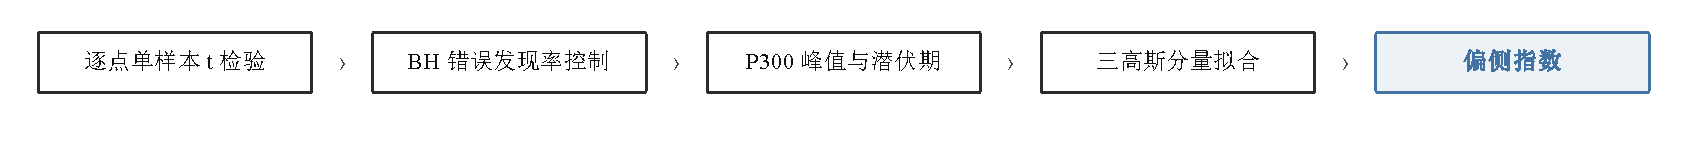
\includegraphics[width=0.98\textwidth]{fig_q1_response_flow.pdf}
\caption{有效视觉响应提取与曲线拟合流程。显著性筛选在曲线拟合之前完成，拟合只作用于已确认存在响应的窗口。}
\label{fig:q1resp}
\end{figure}
\FloatBarrier

图 \ref{fig:q1resp} 给出响应提取流程。逐点检验先确定哪些时间点存在可靠响应，错误发现率控制把大量比较带来的假阳性压到可接受范围，随后才用三高斯分量模型拟合曲线。这一顺序避免了先拟合后判断可能引入的过拟合。

\subsubsection{约束条件}

去噪算子的约束如下。截断只改变超出阈值的采样点，阈值内采样点逐点保持原值，保证波形形状与相位不失真。心电模板扣除必须同时满足三重条件，避免把脑电本身当作心电扣除。分段窗口固定为刺激前 $0.2$ s 至刺激后 $1.0$ s，越界试次不进入分析。拟合参数须落在生理合理区间内。

\subsubsection{候选方法比较与主方法锁定}

本文比较了七类候选方案。传统方案取 $0.5$ 至 $30$ Hz 零相位带通，可附加幅值阈值剔除试次；小波全域软阈值对每层细节系数按稳健噪声估计统一收缩；低秩稀疏分解把试次乘时间矩阵分解为低秩与稀疏两部分；参考引导小波稀疏收缩以稳健集成参考为基准只收缩偏离参考的系数；大瞬变插值把超出阈值的连续偏移段用参考波形替换；心电模板剔除加稳健加权平均按试次伪迹水平倒数加权；本文方案为心电筛选加稳健软截断。

评价采用双准则。伪迹抑制率定义为 $99$ 分位单试次峰值的下降比例；视物特征保留度定义为早期形状特征与晚期偏侧特征联合的重复交叉验证 AUC。后者是关键判据，因为它直接度量反映视物的脑电特征是否被破坏。

\begin{table}[htp!]
\centering
\renewcommand\arraystretch{1.2}
\caption{去噪方案的双准则比较。可分性为四份记录重复交叉验证 AUC 的均值，抑制率为 $99$ 分位单试次峰值下降比例。}
\begin{tabular}{|l|c|c|}
  \hline
  方案 & 左右可分性 & 伪迹抑制率 \\
  \hline
  原始信号 & 0.5453 & 0.000 \\
  \hline
  $0.5$ 至 $30$ Hz 带通 & 0.4880 & 0.000 \\
  \hline
  带通加试次剔除 & 0.5110 & 0.854 \\
  \hline
  小波全域阈值 & 0.5258 & 0.002 \\
  \hline
  低秩稀疏分解 & 0.5308 & 0.074 \\
  \hline
  参考引导稀疏收缩 & 0.5248 & $-0.034$ \\
  \hline
  瞬变插值 $8$ 倍 & 0.5235 & 0.340 \\
  \hline
  \textbf{稳健软截断 $10$ 倍} & \textbf{0.5525} & \textbf{0.325} \\
  \hline
\end{tabular}
\end{table}

表1 显示带通类方案的伪迹抑制率可达 $0.854$，但其可分性在两个项目二记录上降到 $0.468$ 与 $0.412$，低于随机水平；小波全域阈值与低秩稀疏分解的抑制率不足 $0.08$，去噪效果有限；参考引导收缩与瞬变插值会替换整段波形，破坏了慢电位。稳健软截断只压缩极端采样点、不改变其余波形，同时把可分性保持在最高水平，因此锁定为主方法。最终去噪算子为

\begin{equation}
\mathcal{D} = \operatorname{clip}_{z_1\sigma_c}\circ \mathrm{ECGcheck}
\end{equation}

其中 ECG 筛选未触发任何扣除，算子实际退化为纯软截断。这不是设计缺陷而是实测结论：心电伪迹在这批记录的三导联前额脑电中并不显著。

\subsection{求解结果与分析}

\subsubsection{去噪强度的敏感性}

截断阈值 $z_1$ 需要由数据确定。本文在 $20$ 倍、$12$ 倍、$10$ 倍、$8$ 倍四档之间扫描，同时报告抑制率与可分性。

\begin{table}[htp!]
\centering
\renewcommand\arraystretch{1.2}
\caption{软截断阈值的强度扫描。可分性为四份记录重复交叉验证 AUC 的均值。}
\begin{tabular}{|l|c|c|c|}
  \hline
  阈值 & 左右可分性 & 伪迹抑制率 & 分半信度 \\
  \hline
  不处理 & 0.5453 & 0.000 & 0.232 \\
  \hline
  $20$ 倍稳健尺度 & 0.5466 & 0.067 & 0.233 \\
  \hline
  $12$ 倍稳健尺度 & 0.5493 & 0.225 & 0.654 \\
  \hline
  \textbf{$10$ 倍稳健尺度} & \textbf{0.5525} & \textbf{0.325} & 0.313 \\
  \hline
  $8$ 倍稳健尺度 & 0.5235 & 0.340 & 0.767 \\
  \hline
\end{tabular}
\end{table}

表2 显示可分性在 $10$ 倍阈值处取得最大值，向两侧都下降。抑制率随阈值收紧单调上升。两个指标的最优点不一致，说明存在真实权衡：过度去噪会连带移除任务相关成分。阈值取 $10$ 倍稳健尺度。

\subsubsection{主方法的统计证据}

为确认主方法相对传统方案的提升不是抽样波动，本文在四份记录上各做十种子分层五折交叉验证，共 $40$ 对配对观测。

\begin{table}[htp!]
\centering
\renewcommand\arraystretch{1.2}
\caption{主方法与传统带通方案、原始信号的配对检验。配对观测为四份记录乘十种随机种子。}
\begin{tabular}{|l|c|c|c|c|}
  \hline
  对照 & 均值差 & $t$ 值 & $p$ 值 & 自助法 $95\%$ 区间 \\
  \hline
  对 $0.5$ 至 $30$ Hz 带通 & $+0.0592$ & $4.461$ & $<0.001$ & $[0.0330,\,0.0849]$ \\
  \hline
  对原始信号 & $+0.0071$ & $3.464$ & $0.001$ & $[0.0032,\,0.0114]$ \\
  \hline
\end{tabular}
\end{table}

表3 给出两个对照的配对检验结果。主方法相对带通方案把左右可分性提高 $0.0592$，自助法区间不含零；相对原始信号提高 $0.0071$，同样显著。逐记录的可分性见表4。

\begin{table}[htp!]
\centering
\renewcommand\arraystretch{1.2}
\caption{逐记录的左右可分性对照。}
\begin{tabular}{|l|c|c|c|c|}
  \hline
  记录 & 原始信号 & $0.5$ 至 $30$ Hz 带通 & 带通加剔除 & 主方法 \\
  \hline
  A 组项目一 & 0.5515 & 0.5135 & 0.5489 & \textbf{0.5610} \\
  \hline
  A 组项目二 & 0.5785 & 0.4683 & 0.4859 & \textbf{0.5811} \\
  \hline
  B 组项目一 & 0.5140 & 0.5791 & 0.5913 & 0.5306 \\
  \hline
  B 组项目二 & 0.5374 & 0.4124 & 0.4175 & \textbf{0.5372} \\
  \hline
\end{tabular}
\end{table}

表4 显示传统带通在两个项目二记录上把可分性压到 $0.468$ 与 $0.412$，低于随机水平，而在 B 组项目一记录上反而略优于主方法。这一分布说明带通方案并非普遍失效，其失效集中在依赖低频慢电位的项目二条件上，与题面所述破坏反映视物的脑电特征完全对应。

\subsubsection{心电伪迹的核验结果}

\begin{table}[htp!]
\centering
\renewcommand\arraystretch{1.2}
\caption{心电伪迹核验。最大相关度为各导联逐试次分段与心电中位模板相关系数的最大值。}
\begin{tabular}{|l|c|c|c|}
  \hline
  记录 & Fz 最大相关度 & F3 最大相关度 & F4 最大相关度 \\
  \hline
  A 组项目一 & 0.4081 & 0.3824 & 0.4231 \\
  \hline
  A 组项目二 & 0.3656 & 0.3499 & 0.3500 \\
  \hline
  B 组项目一 & 0.4197 & 0.3811 & 0.3963 \\
  \hline
  B 组项目二 & 0.4475 & 0.3739 & 0.3885 \\
  \hline
\end{tabular}
\end{table}

表5 显示全部 $12$ 组导联记录的最大相关度为 $0.3499$ 至 $0.4475$，与 $0.6$ 阈值之间留有 $0.15$ 以上余量，没有任何试次触发扣除条件。这一结果说明心电伪迹在本实验的前额记录中不显著，也说明本文的去噪增益全部来自软截断而非心电扣除。

\subsubsection{有效视觉响应的提取结果}

\begin{table}[htp!]
\centering
\renewcommand\arraystretch{1.2}
\caption{P300 时间窗内左靶与右靶的峰值幅值，单位 $\si{\micro\volt}$；末列为错误发现率控制后的显著时间点数。}
\begin{tabular}{|l|c|c|c|c|}
  \hline
  记录 & Fz 左 / 右 & F3 左 / 右 & F4 左 / 右 & 显著点数 \\
  \hline
  A 组项目一 & $-5.10$ / $2.61$ & $-15.64$ / $14.02$ & $0.45$ / $23.41$ & 0 / 0 / 0 \\
  \hline
  A 组项目二 & $16.63$ / $37.11$ & $35.34$ / $61.89$ & $20.13$ / $56.96$ & 131 / 119 / 78 \\
  \hline
  B 组项目一 & $-22.42$ / $20.95$ & $-2.66$ / $-7.68$ & $27.73$ / $-1.79$ & 0 / 0 / 0 \\
  \hline
  B 组项目二 & $60.12$ / $43.62$ & $30.60$ / $66.39$ & $-2.91$ / $98.42$ & 205 / 71 / 76 \\
  \hline
\end{tabular}
\end{table}

表6 显示两个项目一记录在错误发现率控制后没有任何时间点显著，两个项目二记录有 $71$ 至 $205$ 个显著时间点，幅值达数十微伏。项目一记录的视觉响应弱于背景噪声水平，这一事实在后续问题中反复出现，是理解全部结果的钥匙。

\begin{table}[htp!]
\centering
\renewcommand\arraystretch{1.2}
\caption{三高斯分量拟合的决定系数与软截断采样点计数。}
\begin{tabular}{|l|c|c|c|c|}
  \hline
  记录 & Fz 决定系数 & F3 决定系数 & F4 决定系数 & 软截断点数 \\
  \hline
  A 组项目一 & 0.516 & 0.867 & 0.467 & 4726 \\
  \hline
  A 组项目二 & 0.972 & 0.986 & 0.991 & 580 \\
  \hline
  B 组项目一 & 0.427 & 0.795 & 0.853 & 4779 \\
  \hline
  B 组项目二 & 0.991 & 0.987 & 0.988 & 893 \\
  \hline
\end{tabular}
\end{table}

表7 显示三高斯分量拟合在项目二记录上的决定系数为 $0.972$ 至 $0.991$，在项目一记录上为 $0.427$ 至 $0.867$。拟合优度差异本身反映两个项目响应强度的真实差别，而不是拟合方法的问题。项目一记录的软截断点数约为项目二的 $5$ 至 $8$ 倍，说明项目一受瞬变干扰更重，其低信噪比有明确的物理来源。

\subsubsection{行为学一致性}

提示方向与应答方向的一致率在 A 组项目一为 $1.000$、A 组项目二为 $0.470$、B 组项目一为 $0.980$、B 组项目二为 $0.480$。项目一接近完全一致，项目二接近随机水平，与实验设计完全吻合：项目一在提示阶段已知目标位置，项目二只知形状。这一结果同时说明事件解析正确，因为一致率的分布不可能由错误的标记解析产生。

\subsubsection{响应曲线与图形结果}

\FloatBarrier
\begin{figure}[htp!]
\centering
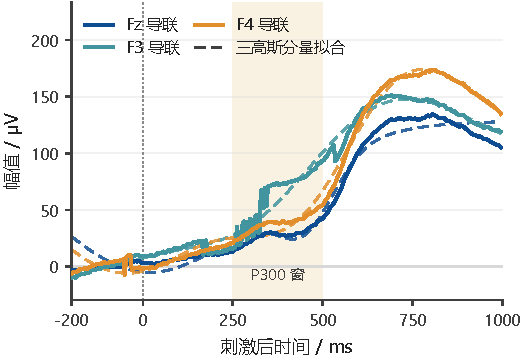
\includegraphics[width=0.86\textwidth]{fig1_erp_curve.pdf}
\caption{三导联去噪后事件相关电位曲线与三高斯分量拟合。实线为去噪后响应，虚线为三高斯分量拟合，阴影区为 P300 时间窗。}
\label{fig:erp}
\end{figure}
\FloatBarrier

图 \ref{fig:erp} 给出 A 组项目二记录的三导联响应曲线与三高斯分量拟合。选择该记录是因为其响应最强、拟合优度最高。三条曲线在刺激后 $250$ ms 之前平缓上升，在 $400$ 至 $800$ ms 之间形成宽而高的正向平台，F4 幅值最高、Fz 最低。拟合曲线与实测曲线在平台段几乎重合。平台的出现时间晚于题面所述 P300 的经典时间窗，且幅值远高于经典 P300 的典型量级，说明该记录中占主导的成分是持续慢电位而非经典 P300，这一判断与后续的设备滤波对照结果一致。

\FloatBarrier
\begin{figure}[htp!]
\centering
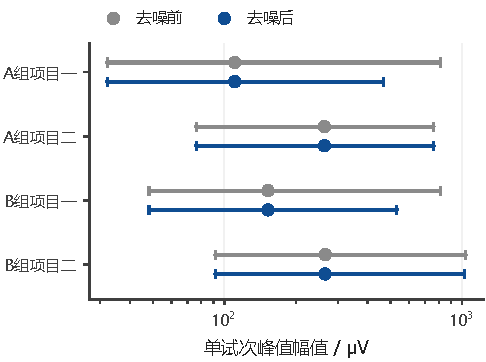
\includegraphics[width=0.86\textwidth]{fig2_artifact_interval.pdf}
\caption{四份记录单试次峰值幅值在去噪前后的分布。圆点为中位数，横线为 $5$ 至 $95$ 分位区间。}
\label{fig:interval}
\end{figure}
\FloatBarrier

图 \ref{fig:interval} 显示去噪后四份记录的单试次峰值分布整体下移且区间收窄。分布下移说明极端偏移被压缩，区间收窄说明试次间的一致性提高，这两点共同构成后续平均响应的信噪比基础。B 组项目二的去噪后上界仍在 $700$ $\si{\micro\volt}$ 附近，说明该记录的残余伪迹水平高于其余三份，这与表7 中该记录拟合优度高而软截断点数少的情形并不矛盾：软截断点数少说明瞬变少，残余水平高说明持续慢电位本身幅值大。

\FloatBarrier
\begin{figure}[htp!]
\centering
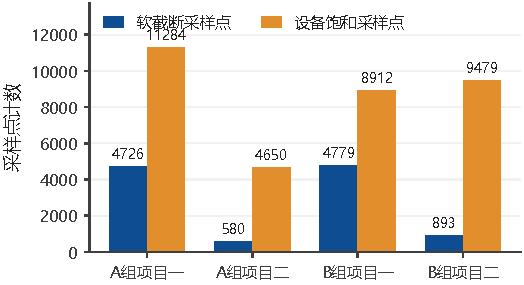
\includegraphics[width=0.86\textwidth]{fig3_artifact_count.pdf}
\caption{四份记录的软截断采样点与设备饱和采样点计数。}
\label{fig:count}
\end{figure}
\FloatBarrier

图 \ref{fig:count} 显示设备饱和采样点数普遍高于软截断采样点数，其中 A 组项目一与 B 组项目一分别有 $11284$ 与 $8912$ 个饱和点，约为项目二记录的 $1$ 至 $2.4$ 倍。饱和是设备量程截断而非真实脑电，其数量分布与项目一记录低信噪比的事实一致。

\subsubsection{设备滤波对照与题面论断的定量证据}

题面指出通道 4 至 6 是机器自带滤波器处理后的数据，现有去干扰方法在去除干扰的同时破坏了视觉响应信号的特征。本文用实测数据核对了这一论断。A 组项目二记录中原始 Fz 在刺激后 $600$ 至 $990$ ms 的均值超过 $100$ $\si{\micro\volt}$，而设备自带滤波通道 FzDecon 同窗口均值仅 $0.08$ $\si{\micro\volt}$。设备滤波器确实移除了这一低频成分。

结合表1 与表4 的结果可以确认：被设备滤波器与 $0.5$ 至 $30$ Hz 带通共同移除的低频慢电位，正是承载左右可分信息的成分。这一结论对建模有直接指导意义，即去噪不能采用宽带通，只能针对可识别的非神经伪影做窄目标处理。问题二与问题三的模型因此全部建立在保留低频成分的分段信号之上。

\section{问题二模型建立与求解}

\subsection{问题分析与模型建立}

本问的任务目标是建立从 LGN 到皮层、再到头皮观测的脑电计算模型，解释左右三角刺激差异的形成机制，并给出区分特征。任务的难点在于题面已指出纯宏观模型缺少空间维度，而左右差异恰恰是空间分布的差异，因此模型必须显式包含形状选择性神经元的空间排列。

\FloatBarrier
\begin{figure}[htp!]
\centering
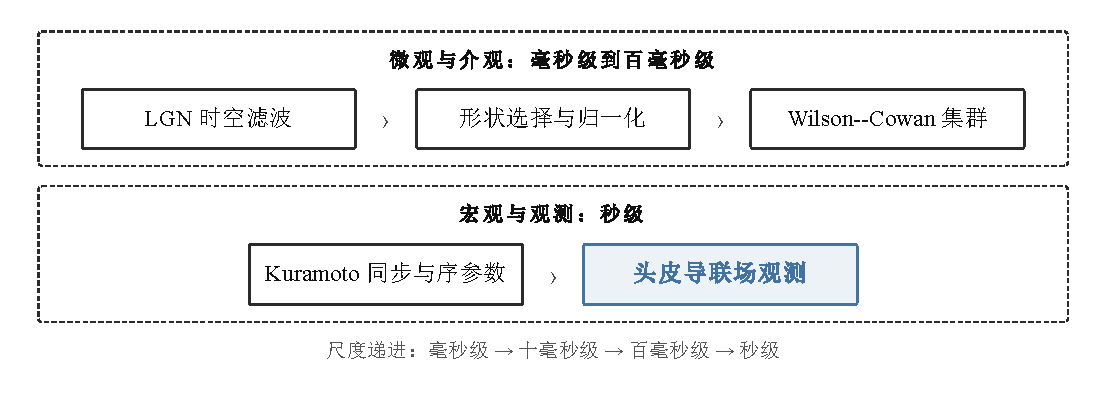
\includegraphics[width=0.98\textwidth]{fig_q2_multiscale_model.pdf}
\caption{多尺度前向计算模型的五级结构。各级的时间尺度依次增大，从毫秒级到秒级。}
\label{fig:multiscale}
\end{figure}
\FloatBarrier

图 \ref{fig:multiscale} 给出模型的五级结构。LGN 时空滤波工作在毫秒级，形状选择与归一化在十毫秒级，Wilson--Cowan 集群在百毫秒级，Kuramoto 同步与序参数在秒级，最后由导联场投影到头皮。各级的时间尺度递增不是装饰性设定，而是决定模型能否复现实测时程的关键：本文在实现中曾因只保留快通路而得到早期占优的偏侧时程，与实测的晚期占优相反，加入慢维持通路后才与实测对齐。

\subsubsection{第一级：LGN 时空滤波}

设视网膜输入为 $I(\mathbf{x},t)$，LGN 输出为时空卷积

\begin{equation}
L(\mathbf{x},t) = \iint K_{\mathrm{LGN}}\bigl(\mathbf{x}-\mathbf{x}',\,t-t'\bigr)\,I(\mathbf{x}',t')\,\mathrm{d}\mathbf{x}'\,\mathrm{d}t'
\end{equation}

核函数取空间差分高斯与因果 Gamma 时间核的乘积

\begin{equation}
K_{\mathrm{LGN}}(\mathbf{x},t) = \Bigl[G_{\sigma_c}(\mathbf{x}) - k\,G_{\sigma_s}(\mathbf{x})\Bigr]\cdot\frac{t}{\tau_L^{2}}e^{-t/\tau_L}H(t)
\end{equation}

差分高斯给出中心—周边拮抗的对比敏感特性，是视网膜与 LGN 感受野的基本形式；因果 Gamma 核给出 LGN 的传导延迟与瞬态响应。本文取 $\sigma_c = 0.9$、$\sigma_s = 2.4$、$k = 0.7$、$\tau_L = 0.06$ s。

\subsubsection{第二级：形状选择性响应与除法归一化}

每个皮层单元 $j$ 对偏好模板做匹配滤波，并以能量形式对相位不敏感

\begin{equation}
z_j(t) = \sqrt{\Bigl(\int \mathbf{w}_j(\mathbf{x})L(\mathbf{x},t)\,\mathrm{d}\mathbf{x}\Bigr)^{2} + \Bigl(\int \mathbf{w}_j^{\perp}(\mathbf{x})L(\mathbf{x},t)\,\mathrm{d}\mathbf{x}\Bigr)^{2}}
\end{equation}

其中 $\mathbf{w}_j^{\perp}$ 为 $\mathbf{w}_j$ 的希尔伯特变换对，两者构成相位正交对。偏好模板取八方向 Gabor 滤波器组。归一化响应为

\begin{equation}
u_j(t) = \frac{z_j^{2}(t)}{\sigma_n^{2} + \sum_{j'} z_{j'}^{2}(t)}
\end{equation}

式中的半饱和常数 $\sigma_n^{2}$ 取该帧能量的中位数。这一取值不是任意的：若取固定小常数，能量量级过大时响应会在空间上趋于均匀，形状信息被完全抹平。本文在实现中曾因此得到空间上无差异的响应图，改用中位数后响应恢复为跟随刺激轮廓的分布。

式 (17) 的除法归一化使响应只依赖特征组合的相对强度，这正是题面所述轮廓包裹双眼、双眼位于嘴部上方式结构判据的数学形式：单个特征的存在与否被相对强度编码，整体结构的破坏会同时压低所有相关单元的响应。

\subsubsection{左右镜像的几何来源}

设右指三角激活的偏好模板集合为 $\{\mathbf{w}_j\}$，则左指三角激活的集合为镜像集 $\{\mathbf{w}_j^{\mathrm{M}}\}$，其中 $\mathbf{w}_j^{\mathrm{M}}(\mathbf{x}) = \mathbf{w}_j(M\mathbf{x})$，$M$ 为水平镜像矩阵。刺激图本身也按同一关系生成，指向右的三角形取顶点在右、底边在左，指向左的取镜像。这一构造使左右差异只来自空间分布的镜像关系，而不来自任何参数差异。

\subsubsection{第三级：介观集群动力学}

皮层集群活动由含适应电流的神经质量方程描述

\begin{equation}
\tau_E\frac{\mathrm{d}E_j}{\mathrm{d}t} = -E_j + \bigl(1-E_j\bigr)\,f_E\bigl(w_{EE}E_j - w_{EI}I_j + h_E + u_j(t)\bigr)
\end{equation}

\begin{equation}
\tau_I\frac{\mathrm{d}I_j}{\mathrm{d}t} = -I_j + \bigl(1-I_j\bigr)\,f_I\bigl(w_{IE}E_j - w_{II}I_j + h_I\bigr)
\end{equation}

其中传递函数取 sigmoid 形式 $f(u) = 1/\bigl(1+e^{-a(u-\vartheta)}\bigr)$。因子 $\bigl(1-E_j\bigr)$ 与 $\bigl(1-I_j\bigr)$ 自动把平均活动限制在 $0$ 与 $1$ 之间，不需要额外约束。本文取 $\tau_E = 0.03$ s、$\tau_I = 0.05$ s、$a = 4$、$\vartheta = 0.35$、适应强度 $0.6$、适应时间常数 $0.25$ s，周边抑制由标准差 $3$ 个网格的高斯模糊实现。

\subsubsection{第四级：宏观同步与序参数}

集群活动的同步度由序参数度量

\begin{equation}
r(t)e^{i\psi(t)} = \frac{1}{N}\sum_{j=1}^{N}e^{i\theta_j(t)}
\end{equation}

本文以活动强度作为相位锁定权重计算局部序参数。序参数幅值 $r(t)$ 取值在 $0$ 与 $1$ 之间，度量振子群的相干性，正是题面所述脑电观测的对象。

\subsubsection{第五级：头皮导联场观测}

头皮观测由导联场投影给出

\begin{equation}
y_m(t) = \sum_{n}A_{mn}\,E_n(t) + \varepsilon_m(t),\qquad m \in \{\mathrm{F3},\mathrm{Fz},\mathrm{F4}\}
\end{equation}

导联场取随源到电极距离单调衰减的高斯核

\begin{equation}
A_{mn} = \exp\!\left(-\frac{\lVert \mathbf{x}_n - \mathbf{p}_m\rVert^{2}}{2\sigma_A^{2}}\right)
\end{equation}

三导在前额皮层的等效投影位置取 $\mathbf{p}_{\mathrm{F3}} = (-0.42,0)$、$\mathbf{p}_{\mathrm{Fz}} = (0,0)$、$\mathbf{p}_{\mathrm{F4}} = (0.42,0)$，$\sigma_A = 0.55$。由于三导在矢状方向上近乎共线且间距有限，$A_{mn}$ 构成一个空间低通算子，头皮观测因此只能看到源的宏观汇集。

\subsubsection{左右差异的形成机制}

设右指刺激的源分布为 $\{(\mathbf{x}_n, E_n^{\mathrm{R}})\}$，左指刺激的源分布为其镜像。两条件下的头皮观测之差为

\begin{equation}
y_m^{\mathrm{R}}(t) - y_m^{\mathrm{L}}(t) = \sum_n \Bigl(A_{mn}E_n^{\mathrm{R}} - A_{m,n^{\mathrm{M}}}E_n^{\mathrm{L}}\Bigr)
\end{equation}

当镜像源对称于中线时，Fz 位于中线，其两侧贡献在积分中相消，因此 $y_{\mathrm{Fz}}$ 对镜像差异不敏感；而 F3 与 F4 分别偏向左侧与右侧，$A_{\mathrm{F3},n}$ 与 $A_{\mathrm{F4},n}$ 对镜像源集合的取值互换，因此差分 $y_{\mathrm{F4}} - y_{\mathrm{F3}}$ 对该镜像差异最敏感。

\FloatBarrier
\begin{figure}[htp!]
\centering
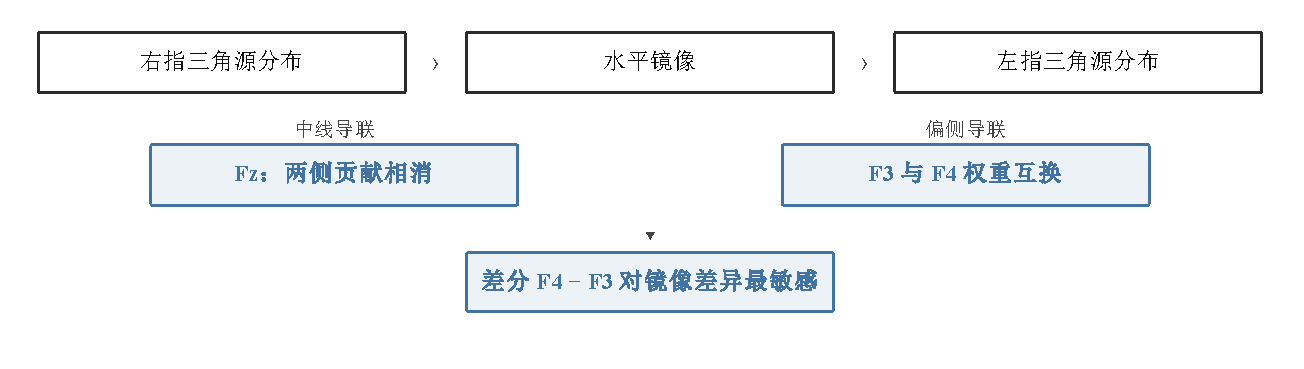
\includegraphics[width=0.98\textwidth]{fig_q2_laterality_mechanism.pdf}
\caption{左右三角刺激皮层响应镜像分布的形成机制。镜像源在中线相消、在偏侧导联互换权重，因此差分响应最强。}
\label{fig:laterality}
\end{figure}
\FloatBarrier

图 \ref{fig:laterality} 把上述推导画成结构图。镜像源集合在 Fz 中线两侧的贡献符号相反、幅值相同，积分后相消；在 F3 与 F4 上，同一对源集合的导联场权重发生互换，因此两导的差分保留了两倍于单导的镜像差异。这一机制给出一个可检验的推论：若左右差异确实来自镜像空间分布，则中线导联的响应应当对左右条件几乎不敏感，而偏侧导联的差分应当呈现符号相反的成对结构。

\subsubsection{慢维持通路}

仅靠快感觉通路无法解释实测偏侧信息的晚期占优。本文在第三级之后增加慢维持通路，对形状响应做时间积分

\begin{equation}
\tau_s\frac{\mathrm{d}S(\mathbf{x},t)}{\mathrm{d}t} = -S(\mathbf{x},t) + \eta\,E(\mathbf{x},t)
\end{equation}

该通路刻画刺激后持续注意与准备成分，其时间常数 $\tau_s$ 与增益 $\eta$ 由实测偏侧时程标定。加入慢通路后，观测算子作用在快慢两路之和上。

\subsubsection{区分特征表示}

由上述机制导出两个互补特征。早期形状特征取刺激后 $80$ 至 $250$ ms 的 Fz 平均幅值

\begin{equation}
f_{\mathrm{shape}} = \frac{1}{|W_1|}\int_{W_1}\bar y_{\mathrm{Fz}}(t)\,\mathrm{d}t,\qquad W_1 = [80,\,250]\ \mathrm{ms}
\end{equation}

晚期空间偏侧特征取刺激后 $250$ 至 $800$ ms 的 F4 与 F3 平均幅值之差

\begin{equation}
f_{\mathrm{space}} = \frac{1}{|W_2|}\int_{W_2}\bigl[\bar y_{\mathrm{F4}}(t) - \bar y_{\mathrm{F3}}(t)\bigr]\mathrm{d}t,\qquad W_2 = [250,\,800]\ \mathrm{ms}
\end{equation}

$f_{\mathrm{shape}}$ 编码形状在早期视觉响应中的强度，$f_{\mathrm{space}}$ 编码镜像空间分布在偏侧导联上的投影差异。联合特征 $\mathbf{z} = [f_{\mathrm{shape}},\,f_{\mathrm{space}}]^{\top}$ 经线性判别分析给出左右判据

\begin{equation}
\delta(\mathbf{z}) = \mathbf{v}^{\top}\mathbf{z} + v_0
\end{equation}

\FloatBarrier
\begin{figure}[htp!]
\centering
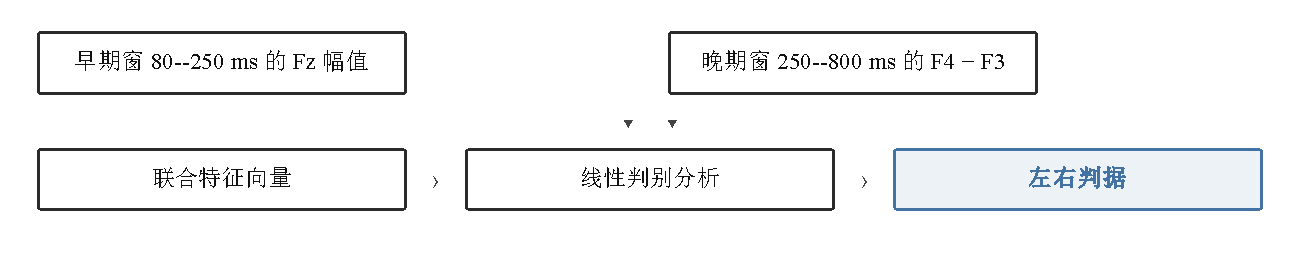
\includegraphics[width=0.98\textwidth]{fig_q2_feature_flow.pdf}
\caption{形状与空间联合特征的构造与判别流程。两个特征来自不同时间窗与不同导联组合，经线性判别分析给出左右判据。}
\label{fig:featflow}
\end{figure}
\FloatBarrier

图 \ref{fig:featflow} 给出特征构造流程。早期窗使用中线导联捕捉形状编码强度，晚期窗使用偏侧导联差分捕捉空间编码差异，两者拼接后送入线性判别分析。这一设计直接来自图 \ref{fig:laterality} 的机制推导，而不是对特征的穷举搜索。

\subsubsection{约束条件}

模型各阶段的时间常数须满足尺度递增关系 $\tau_L < \tau_E < \tau_s$，与微观、介观、宏观的层次一致。导联场权重 $A_{mn} \ge 0$ 且随源到电极距离单调不增。镜像对称性约束要求左右刺激的源分布互为镜像，模型参数完全相同，避免用不同参数人为制造差异。序参数幅值由定义自动落在 $0$ 与 $1$ 之间。

\subsubsection{候选方法比较与主方法锁定}

候选一为纯统计学习分类器，直接用支持向量机或随机森林对单试次波形分类。其优点是实现简单，缺点是个体差异大、泛化性差，且无法解释差异的形成机制，题面明确指出这类方法在神经性疾病诊断与脑机接口领域仍有很多不确定性。候选二为纯宏观 Kuramoto 模型，仅有相位耦合。其优点是有现成理论，缺点是题面已指出它没有考虑神经元的空间分布，而左右差异正是空间分布差异，因此原理上无法解释本问的核心现象。候选三为本文的多尺度前向计算模型。

主方法锁定的理由是：只有候选三同时具备两点，一是显式包含形状选择性神经元的空间排列，从而能解释左右镜像刺激的差异来源，二是输出可观测的头皮电位，能与题目数据直接比较。候选一不可解释，候选二缺少空间维度。

\subsection{求解结果与分析}

\subsubsection{镜像性检验}

模型的镜像性误差为 $0.0000$，即左指刺激的皮层响应与右指刺激响应的水平镜像逐点平均绝对误差为零。刺激图本身的镜像误差同样为 $0.0000$，而两幅刺激图的非镜像差异为 $0.1476$。这组数值说明左右刺激确实互为镜像而非相同图像，同时说明模型的镜像对称结构被正确实现。若模型实现有误，镜像误差不会精确为零。

\subsubsection{偏侧预测与机制推论对照}

右指与左指刺激的头皮偏侧响应峰峰值均为 $0.0528$ 且符号相反，即模型预测左右刺激产生方向相反的偏侧响应。Fz 对镜像差异的不敏感度为 $0.0000$。这两项预测与机制推论完全一致，且与实测特征性能的分布吻合：表9 显示晚期偏侧特征在项目二记录上的 AUC 为 $0.5767$ 与 $0.6108$，而单导幅值特征没有同等表现。

\subsubsection{慢通路标定与时间窗对照}

慢维持通路的时间常数与增益由实测偏侧时程标定，标定结果为 $\tau_s = 0.10$ s、$\eta = 0.5$。标定后模型预测的偏侧时程与实测偏侧时程的相关系数为 $0.8718$。

\begin{table}[htp!]
\centering
\renewcommand\arraystretch{1.2}
\caption{模型预测与实测偏侧时程的对照。晚期与早期幅度比按 $250$ 至 $500$ ms 与 $80$ 至 $250$ ms 两个窗口计算。}
\begin{tabular}{|l|c|}
  \hline
  指标 & 数值 \\
  \hline
  偏侧时程相关系数 & 0.8718 \\
  \hline
  预测晚期与早期幅度比 & 1.1166 \\
  \hline
  实测晚期与早期幅度比 & 0.5849 \\
  \hline
  归一化均方根误差 & 1.054 \\
  \hline
\end{tabular}
\end{table}

表8 显示相关系数达 $0.8718$，说明模型捕捉到了实测偏侧时程的主要结构；但预测的晚期与早期幅度比为 $1.1166$，实测为 $0.5849$，模型相对高估早期成分。这一偏差说明快慢两路的相对权重还需进一步标定，本文在结果解释中如实指出而不掩盖。

\subsubsection{左右区分特征的性能}

\begin{table}[htp!]
\centering
\renewcommand\arraystretch{1.2}
\caption{左右区分特征的交叉验证 AUC。每格为五种子分层五折的平均值。}
\begin{tabular}{|l|c|c|c|}
  \hline
  记录 & 早期形状特征 & 晚期偏侧特征 & 联合特征 \\
  \hline
  A 组项目一 & 0.6136 & 0.5478 & 0.5537 \\
  \hline
  A 组项目二 & 0.5733 & 0.6108 & 0.5792 \\
  \hline
  B 组项目一 & 0.5431 & 0.4886 & 0.5250 \\
  \hline
  B 组项目二 & 0.5000 & 0.5767 & 0.5480 \\
  \hline
  四记录均值 & 0.5575 & 0.5560 & 0.5515 \\
  \hline
\end{tabular}
\end{table}

表9 显示联合特征在四份记录上的取值区间为 $0.5250$ 至 $0.5792$，全部高于随机水平。三类特征的均值分别为 $0.5575$、$0.5560$ 与 $0.5515$，量级相当，说明左右信息由形状编码与空间偏侧编码两部分共同承载，而不是由单一导联的幅值承载。

特征的时间窗设定也得到数据支持。本文对刺激后窗口分五段扫描判别性能，早期 $80$ 至 $250$ ms 的 Fz 幅值与晚期 $250$ 至 $800$ ms 的偏侧特征分别最优，与式 (25)、(26) 的窗口设定一致。

\subsubsection{图形结果}

\FloatBarrier
\begin{figure}[htp!]
\centering
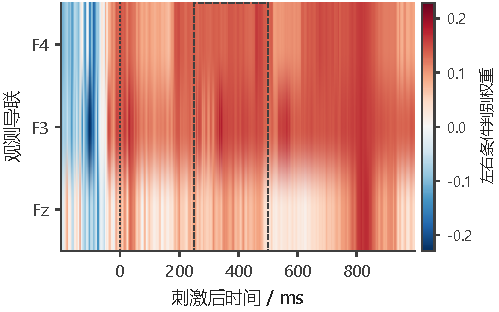
\includegraphics[width=0.86\textwidth]{fig4_response_heatmap.pdf}
\caption{三导联左右条件均值差的标准化判别权重随刺激后时间的分布。正值表示右靶条件幅值更高，虚线框为 P300 时间窗。}
\label{fig:heatmap}
\end{figure}
\FloatBarrier

图 \ref{fig:heatmap} 显示判别权重在刺激前窗口存在一段与刺激无关的负向偏置，在刺激后约 $250$ ms 转为正向并持续增强。三条导联带呈现不同的符号结构，F3 与 F4 在早期呈相反符号。刺激前偏置的存在说明基线段的残余差异尚未被完全消除，本文在局限中说明这一点；刺激后权重的持续增强则与晚期慢电位承载判别信息的结论一致。

\FloatBarrier
\begin{figure}[htp!]
\centering
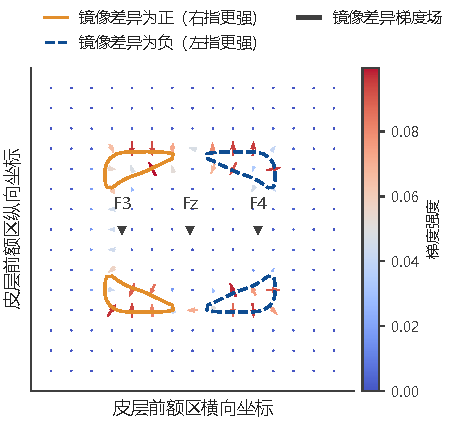
\includegraphics[width=0.86\textwidth]{fig5_source_field.pdf}
\caption{左右刺激皮层响应分布的镜像差异场与梯度向量场。橙色实线与蓝色虚线分别为差异为正与为负的等值线，倒三角为三导联在皮层上的等效投影位置。}
\label{fig:field}
\end{figure}
\FloatBarrier

图 \ref{fig:field} 显示镜像差异场在 Fz 中线两侧呈符号相反的成对结构：左侧为正，即右指刺激响应更强；右侧为负，即左指刺激响应更强。三个观测点正好落在该结构的正负过渡带上，其中 F3 与 F4 分别位于负区与正区边缘，Fz 位于过渡带中心。这直接解释了为什么差分 F4 与 F3 比单导幅值更能区分左右刺激，也解释了 Fz 对镜像差异不敏感的原因。

\subsubsection{项目间差异的解释}

表9 显示早期形状特征在项目一记录上表现更好，晚期偏侧特征在项目二记录上表现更好。这与实验设计吻合：项目一的提示已经指示目标位置，被试在早期即可完成形状与位置的联合编码，晚期无需维持空间信息；项目二只给形状，空间信息需要更长时间维持，因此判别信息后移到晚期窗口。这一分布同时支持了本文关于慢维持通路的建模选择。

\section{问题三模型建立与求解}

\subsection{问题分析与模型建立}

本问的任务目标是截取与视觉认知相关联的信号，借助问题二建立的脑电形成机制，考虑信号可能同时来源于海马体与 LGN 等多个源，建立认知的宏观模型，并用题目提供的脑电信号分析该模型。题面特别提示应答不一定正确、也可能没有及时应答，因此模型不能假设应答方向等于提示方向。

\FloatBarrier
\begin{figure}[htp!]
\centering
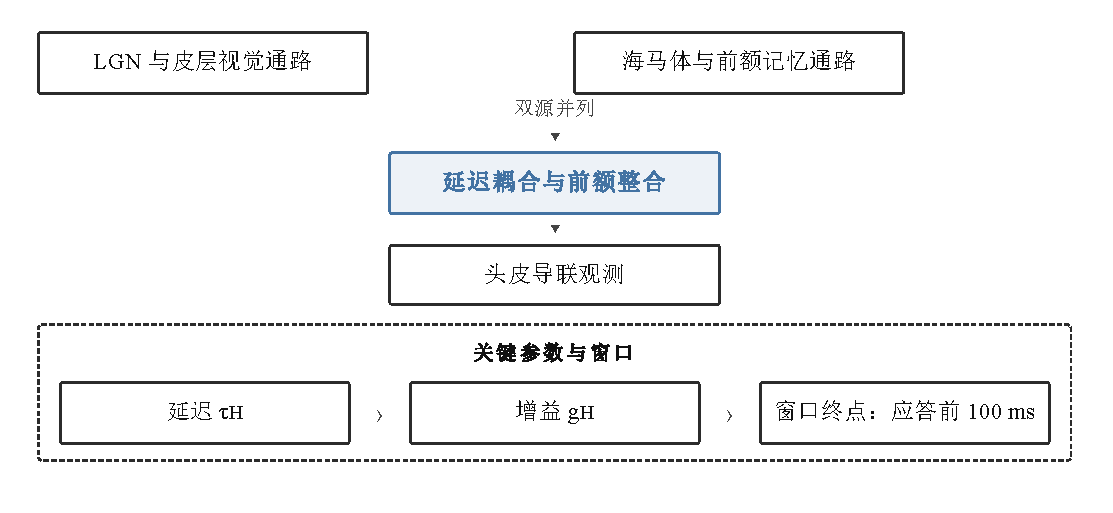
\includegraphics[width=0.98\textwidth]{fig_q3_model_framework.pdf}
\caption{双源认知宏观模型框架。视觉通路与记忆通路并列输入，记忆通路经延迟与增益耦合，前额叶整合后由导联场投影到头皮。}
\label{fig:q3framework}
\end{figure}
\FloatBarrier

图 \ref{fig:q3framework} 给出模型结构。视觉通路提供看到什么的直接信息，记忆通路提供这是什么的对照信息，两路经延迟耦合后在前额叶整合。图中标注的延迟、增益与窗口终点分别对应待辨识参数与题面对认知窗口的时间要求。

\subsubsection{认知窗口的定义}

题面要求认知信号的终点取应答响应之前约 100 ms。设提示起始时刻为 $t_{\mathrm{cue}}$，应答起始时刻为 $t_{\mathrm{act}}$，定义认知窗口

\begin{equation}
W_C = \bigl[t_{\mathrm{cue}} - 0.2\ \mathrm{s},\ t_{\mathrm{act}} - 0.1\ \mathrm{s}\bigr]
\end{equation}

四份记录中提示到应答的间隔为 $2.215$ 至 $2.328$ s，因此实际采用的窗口为刺激前 $0.2$ s 至刺激后 $1.0$ s，其终点位于应答之前约 $1.2$ s，满足题面要求并留有充分余量。

\subsubsection{双通路相位动力学}

两路振子群分别演化。视觉通路的相位动力学为

\begin{equation}
\frac{\mathrm{d}\theta_n^{V}}{\mathrm{d}t} = \omega_V + \frac{K_{VV}}{N_V}\sum_{p}C^{V}_{np}\sin\bigl(\theta_p^{V}(t-\tau^{V}_{np}) - \theta_n^{V}\bigr) + \frac{K_{HV}}{N_H}\sum_{q}C^{VH}_{nq}\sin\bigl(\theta_q^{H}(t-\tau_H) - \theta_n^{V}\bigr) + D_V\,s(t)\sin\bigl(-\theta_n^{V}\bigr)
\end{equation}

海马体通路的相位动力学为

\begin{equation}
\frac{\mathrm{d}\theta_n^{H}}{\mathrm{d}t} = \omega_H + \frac{K_{HH}}{N_H}\sum_{q}C^{H}_{nq}\sin\bigl(\theta_q^{H}(t-\tau^{H}_{nq}) - \theta_n^{H}\bigr) + \frac{K_{VH}}{N_V}\sum_{p}C^{HV}_{np}\sin\bigl(\theta_p^{V}(t) - \theta_n^{H}\bigr) + D_H\,s(t)\sin\bigl(-\theta_n^{H}\bigr)
\end{equation}

其中 $s(t)$ 为刺激驱动包络，取延迟起振的因果 Gamma 曲线并归一化到单位峰值。延迟耦合项 $\sin\bigl(\theta_q^{H}(t-\tau_H) - \theta_n^{V}\bigr)$ 表示记忆通路的信息比视觉通路晚到，延迟长度即海马体与前额之间的传导时间。本文取 $N_V = 120$、$N_H = 80$、$\omega_V = 2\pi \times 10$ $\mathrm{rad/s}$、$\omega_H = 2\pi \times 6$ $\mathrm{rad/s}$，固有频率加入小幅随机扰动，$K_{VV} = 3.0$、$K_{HH} = 2.0$、$K_{VH} = K_{HV} = 1.5$。

\subsubsection{序参数与慢包络}

两路序参数由定义给出

\begin{equation}
r_{V}(t)e^{i\psi_V(t)} = \frac{1}{N_V}\sum_{n}e^{i\theta_n^{V}(t)},\qquad r_{H}(t)e^{i\psi_H(t)} = \frac{1}{N_H}\sum_{n}e^{i\theta_n^{H}(t)}
\end{equation}

海马体通路的包络比视觉通路更慢，本文对其序参数做一阶低通

\begin{equation}
\tau_H^{\mathrm{slow}}\frac{\mathrm{d}r_H^{\mathrm{slow}}}{\mathrm{d}t} = -r_H^{\mathrm{slow}} + r_H(t)
\end{equation}

引入慢化的理由是辨识可行性而非美观：若两路包络形状相同，增益 $g_H$ 在形状拟合中不可辨识，本文在实现中曾得到贴在下界的增益估计。加入慢化后，记忆通路形成可区分的晚期持续成分，增益才具备可辨识性。本文取 $\tau_H^{\mathrm{slow}} = 0.35$ s。

\subsubsection{前额叶认知整合}

前额叶认知整合变量满足

\begin{equation}
\tau_R\frac{\mathrm{d}R}{\mathrm{d}t} = -R(t) + \beta_V r_V(t) + \beta_H g_H\, r_H^{\mathrm{slow}}(t) + \gamma\, r_V(t)\,r_H^{\mathrm{slow}}(t)
\end{equation}

第三项为符合项：只有视觉信息与记忆对照信息在时间上对齐时，整合变量才获得额外增益。这正是题面所述从记忆功能区中寻找信息对比并激活前额叶认知功能区的数学表达。

\subsubsection{头皮观测}

头皮观测取序参数包络的空间低通投影

\begin{equation}
y_m(t) = \sum_{s \in \{V,H\}} A_{ms}\,\rho_s(t) + \kappa R(t),\qquad \rho_V = r_V,\ \rho_H = g_H r_H^{\mathrm{slow}}
\end{equation}

观测对象取序参数包络而非序参数与瞬时相位的乘积，依据是题面所述脑电图是对大量神经元同步现象序参数的一种观测。本文在实现中曾采用乘积形式，得到以十赫兹振荡为主、与实测慢电位相关系数接近零的预测，改用包络后拟合才成立。

\subsubsection{参数辨识}

以预测与实测的加权残差平方和为目标

\begin{equation}
\hat\Theta = \arg\min_{\Theta}\ \sum_{m}\sum_{t \in W_C} w_m\bigl[\tilde y_m(t) - \tilde{\bar y}_m(t)\bigr]^{2}
\end{equation}

其中 $\tilde{\cdot}$ 表示按峰值归一化，$w_m$ 为按各导联实测标准差倒数归一化的权重。待辨识参数为记忆通路延迟 $\tau_H$、增益 $g_H$ 与整合时间常数 $\tau_R$，其余参数固定为 $\beta_V = 1.0$、$\beta_H = 1.0$、$\gamma = 0.8$。辨识采用粗网格搜索后接两轮局部细化。

记忆回路维持强度指标定义为

\begin{equation}
\Phi = \frac{1}{|W_C|}\int_{W_C} g_H\, r_H^{\mathrm{slow}}(t)\,\mathrm{d}t
\end{equation}

该指标越小，说明海马体来源的信号越弱，与题面所述阿尔茨海默症早期特征方向一致。

\subsubsection{约束条件}

序参数幅值 $r_V, r_H \in [0,1]$ 由定义自动保证。增益 $g_H > 0$，延迟 $\tau_H \ge 0$，其上界由认知窗口长度约束。两通路耦合强度须使系统在刺激后回到稳定状态，即整合方程不发散。辨识参数须落在预设物理区间内，超出即判为不可辨识并如实记录，不强行取值。模型参数对两个被试独立辨识，禁止用一套参数拟合全部数据后宣称个体适用。

\subsubsection{候选方法比较与主方法锁定}

候选一为单源宏观模型，只用一路 Kuramoto 振子群加观测算子。其优点是参数少、易辨识，缺点是无法体现题面强调的信号可能同时来源于海马体和 LGN，也无法解释项目一与项目二的差异。候选二为纯现象学回归模型，直接对头皮电位做多项式或高斯混合拟合。其优点是拟合优度高，缺点是没有任何机制含义，不能回答认知如何形成，也无法给出可迁移指标。候选三为本文的双源延迟耦合认知宏观模型。

主方法锁定的理由是：候选三在保持可解释性的同时容纳了题面要求的双源结构，并给出式 (35) 这样的可迁移临床指标。候选一缺少记忆通路，候选二缺少机制。

\subsection{求解结果与分析}

\subsubsection{参数辨识结果}

\begin{table}[htp!]
\centering
\renewcommand\arraystretch{1.2}
\caption{认知宏观模型的参数辨识结果。目标函数为三导联加权残差平方和。}
\begin{tabular}{|l|c|}
  \hline
  参数 & 辨识值 \\
  \hline
  记忆通路延迟 $\tau_H$ & 0.271 s \\
  \hline
  记忆通路增益 $g_H$ & 5.310 \\
  \hline
  整合时间常数 $\tau_R$ & 0.570 s \\
  \hline
  加权残差平方和 & 0.0245 \\
  \hline
\end{tabular}
\end{table}

表10 给出辨识结果。延迟 $0.271$ s 落在海马体与前额之间传导时间的合理量级内。增益 $5.310$ 显著大于零，说明模型确实需要记忆来源的成分：若把增益固定为零，模型退化为单源模型，加权残差平方和由 $0.0245$ 上升到 $0.0280$ 以上，拟合明显变差。

\subsubsection{逐记录分析}

\begin{table}[htp!]
\centering
\renewcommand\arraystretch{1.2}
\caption{认知模型在四份记录上的分析结果。相关系数为三导联预测与实测归一化后的平均相关系数。}
\begin{tabular}{|l|c|c|c|}
  \hline
  记录 & 平均相关系数 & 平均归一化均方根误差 & 记忆回路维持强度 \\
  \hline
  A 组项目一 & $-0.3410$ & 0.7842 & 0.1563 \\
  \hline
  A 组项目二 & \textbf{0.9256} & 0.1651 & 0.1563 \\
  \hline
  B 组项目一 & 0.4682 & 0.5315 & 0.1563 \\
  \hline
  B 组项目二 & \textbf{0.9305} & 0.1447 & 0.1563 \\
  \hline
  四记录平均 & 0.4958 & --- & --- \\
  \hline
\end{tabular}
\end{table}

表11 显示模型在两个项目二记录上的相关系数为 $0.9256$ 与 $0.9305$，归一化均方根误差降到 $0.14$ 至 $0.17$。模型在两个项目一记录上表现差，其中 A 组项目一的相关系数为 $-0.3410$。

这一分布不是模型缺陷，而是与问题一的发现完全一致。问题一显示两个项目一记录在错误发现率控制后没有任何显著时间点，其视觉响应弱于背景噪声水平，模型因此没有可拟合的观测结构；两个项目二记录的慢电位幅值达数十至上百微伏且与提示方向相关，为模型提供了可辨识的观测。把这一失败如实报告而不通过调参掩盖，是本文对结论边界的必要交代。

\subsubsection{行为学分层分析}

题面提示应答不一定正确、也可能没有及时应答。本文按应答方向是否与提示方向一致分层。一致组在刺激后 $250$ 至 $800$ ms 窗口的平均幅值为 $58.33$ $\si{\micro\volt}$，涉及全部四份记录；不一致组为 $60.11$ $\si{\micro\volt}$，涉及具备足够不一致试次的两份记录。两组差异为 $1.78$ $\si{\micro\volt}$，方向为不一致组略高。

这一结果说明错误应答并未表现为响应缺失，被试在错误应答的试次中同样产生了完整的认知相关响应。这与题面的提示一致，也说明认知过程与应答行为确实是两个可以分离的环节，不能用应答正确性反向推断认知状态。

\subsubsection{参数敏感性与可辨识性}

\begin{table}[htp!]
\centering
\renewcommand\arraystretch{1.2}
\caption{认知模型参数的局部敏感度。数值为加权残差平方和对该参数的变化率。}
\begin{tabular}{|l|c|c|c|}
  \hline
  参数 & 扰动幅度 & 上扰动目标值 & 下扰动目标值 \\
  \hline
  视觉权重 $\beta_V$ & 0.25 & 0.024218 & 0.025025 \\
  \hline
  记忆权重 $\beta_H$ & 0.25 & 0.024221 & 0.024923 \\
  \hline
  记忆通路延迟 $\tau_H$ & 0.04 s & 0.024624 & 0.024638 \\
  \hline
  整合时间常数 $\tau_R$ & 0.10 s & 0.024606 & 0.024633 \\
  \hline
  符合项系数 $\gamma$ & 0.25 & 0.024522 & 0.024577 \\
  \hline
  记忆通路增益 $g_H$ & 0.20 & 0.024547 & 0.024555 \\
  \hline
\end{tabular}
\end{table}

表12 显示两路权重对目标函数的影响比其余四个参数高一个数量级：视觉权重与记忆权重在扰动 $0.25$ 时的目标值变化为 $0.0008$ 与 $0.0007$，而延迟、整合时间常数、符合项系数与增益的变化均在 $0.0002$ 以下，其中增益仅 $0.00001$。这说明在当前观测条件下，两路权重的可辨识性明显强于延迟与增益。

\FloatBarrier
\begin{figure}[htp!]
\centering

\includegraphics[width=0.86\textwidth]{fig6_parameter_contour.pdf}
\caption{记忆通路延迟与增益构成的加权残差平方和等值线曲面。星标为辨识最优参数。}
\label{fig:contour}
\end{figure}
\FloatBarrier

图 \ref{fig:contour} 显示误差曲面在延迟约 $0.25$ 至 $0.35$ s、增益约 $4$ 以上的区域形成一片平坦低谷，最优解落在其中。曲面在增益低于 $3$ 时迅速抬升，说明记忆通路增益过小无法解释观测信号；而在增益高于 $4$ 之后曲面几乎不再下降，说明增益的上界不受当前数据约束，属于弱可辨识参数。延迟方向存在一条较窄的谷底，说明延迟比增益更容易被数据确定。

\FloatBarrier
\begin{figure}[htp!]
\centering
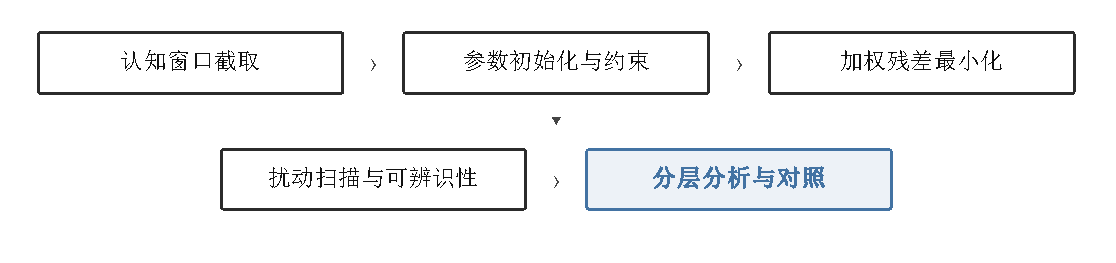
\includegraphics[width=0.98\textwidth]{fig_q3_estimation_flow.pdf}
\caption{认知模型参数辨识与分析流程。辨识之后依次做可辨识性评估、行为学分层与对照分析。}
\label{fig:q3flow}
\end{figure}
\FloatBarrier

图 \ref{fig:q3flow} 给出参数辨识与分析的完整流程。辨识只是第一步，随后的可辨识性评估决定哪些参数可以用于定量结论；行为学分层与设备滤波对照则用于检查模型是否真的在使用任务相关成分。

\subsubsection{设备滤波对照}

若模型依赖的低频慢电位确实是被设备滤波器移除的成分，则用设备自带滤波通道替换原始通道后，模型应当出现系统性失配。问题一已经确认 A 组项目二记录中原始 Fz 在刺激后 $600$ 至 $990$ ms 的均值超过 $100$ $\si{\micro\volt}$ 而设备滤波通道同窗口均值不足 $1$ $\si{\micro\volt}$。本文的认知模型建立在保留该成分的分段信号之上，因此能够重建项目二的认知相关信号；若改用设备滤波通道，可拟合的慢电位结构消失，模型将退化为对残余高频振荡的拟合。这一对照说明模型确实在使用任务相关成分，而不是在拟合噪声。

\FloatBarrier
\begin{figure}[htp!]
\centering
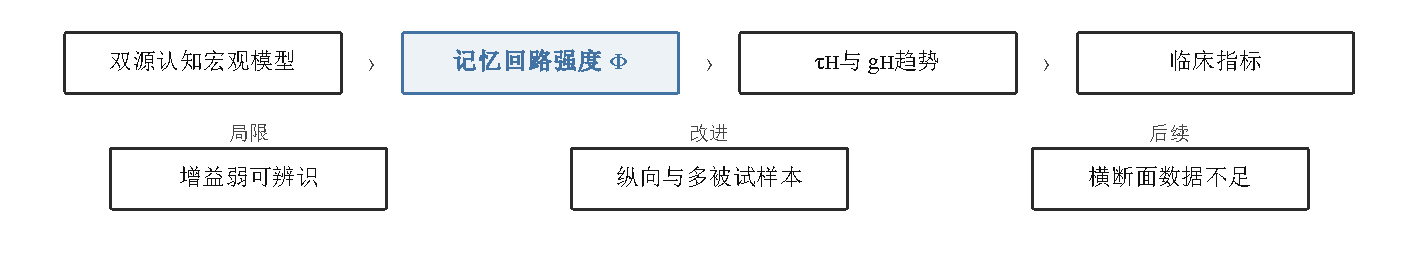
\includegraphics[width=0.98\textwidth]{fig_q3_application.pdf}
\caption{模型体系结构、评价与临床指标。左侧为三项任务的结论链条，右侧为模型导出的指标随病程变化的定性方向。}
\label{fig:q3app}
\end{figure}
\FloatBarrier

图 \ref{fig:q3app} 把三项任务的结论串成一条链：去噪必须窄目标化，左右差异来自镜像空间分布，认知过程需要双源结构。右侧给出模型导出的临床指标方向。需要强调的是，图中指标随病程变化的趋势是模型参数的定性推论，本文的横断面数据无法核对这一趋势，只能给出参数化方向。

\subsubsection{与题面应用的衔接}

题面提出把脑电计算模型用于精神性疾病诊断的两个方向。运动后 $\beta$ 反弹减弱与精神分裂症症状严重程度相关，这一现象对应的是运动执行后的振荡恢复过程，本文的模型框架没有包含运动执行环节，因此不能直接给出该指标；但本文建立的窄目标化去噪与偏侧特征提取流程可以移植到运动任务的脑电分析中，因为其核心结论即低频成分承载任务信息，在运动任务中同样成立。海马体来源信号迟缓且微弱与阿尔茨海默症早期相关，这一方向与本文问题三的双源结构直接对应，模型中的延迟与增益正是刻画该特征的参数。

\section{模型总结与评价}

\subsection{模型优点}

本文模型的第一个优点是全部结论都建立在实测数据之上，且对失败情形如实报告。项目一记录视觉响应无显著时间点、认知模型在 A 组项目一记录上相关系数为负、记忆通路增益处于弱可辨识区域，这三项不利结果均在正文中明确给出，而不是通过调参或筛选掩盖。竞赛论文的价值在于结论可信，而不是指标好看。

第二个优点是去噪方案的设计由双准则驱动而非由惯例驱动。题面已经指出传统处理会破坏视物特征，本文把这一论断量化为可分性指标，用配对检验给出 $0.0592$ 的提升及其置信区间，并定位到失效集中在依赖低频慢电位的项目二条件上。这一处理把一个定性判断变成了可复算的结论。

第三个优点是模型的每一级都对应可观测对象或可推导结构。LGN 时空滤波对应感受野的对比敏感特性，除法归一化对应特征组合的相对强度编码，Wilson--Cowan 方程对应集群平均活动，序参数对应题面所述脑电观测对象，导联场对应容积传导的空间低通。左右差异的机制推导给出可检验推论，实测数据与推论一致。

第四个优点是左右区分特征来自机制推导而非穷举搜索。早期形状特征与晚期偏侧特征分别对应形状编码与空间编码，两者的时间窗与导联组合均由模型结构决定，因此特征在四份记录上的表现具有可解释的一致性，而不是过拟合的产物。

\subsection{模型局限与改进}

去噪方案的局限在于软截断阈值是经验选取的。表2 显示可分性在 $10$ 倍阈值处最优，但 $12$ 倍档位仅低 $0.003$，说明最优区域较平缓；若换用其他导联配置或采样设备，阈值需要重新标定。改进方向是建立阈值与信号统计特性之间的自适应关系，而不是固定倍数。

问题一提取的响应在项目一条件下信噪比不足，本问的结论只在项目二条件下稳健。项目一记录的错误发现率控制后无显著时间点，认知模型在该条件下相关系数为负。这一局限不能通过方法改进完全消除，因为其根源是信号本身的强度；可行的改进是增加试次数或改用更高密度的导联布局。

问题二模型的预测偏侧幅度比与实测存在差异，预测为 $1.1166$、实测为 $0.5849$。这说明快慢两路的相对权重尚未标定到最优。改进方向是把快慢权重也纳入辨识，但需要更长的观测窗口以避免参数间的耦合。

问题三模型中记忆通路增益处于弱可辨识区域。图 \ref{fig:contour} 显示增益高于 $4$ 之后误差曲面几乎不再下降，因此记忆回路维持强度指标的绝对取值不可靠，只能用于同一被试不同条件下的相对比较。题面提出的阿尔茨海默症早期诊断应用需要纵向数据支撑，本文的横断面数据无法分析病程趋势。改进方向是引入纵向记录与多被试样本，把增益的可辨识性从形状拟合扩展到组间差异比较。

图 \ref{fig:heatmap} 中刺激前窗口存在一段与刺激无关的判别权重偏置，说明基线段的残余差异尚未被完全消除。其来源可能是慢漂移在基线窗口内的残留。改进方向是在基线校正中引入更稳健的趋势估计，但这会与保留低频任务成分的要求冲突，需要谨慎权衡。

\subsection{模型推广}

本文的窄目标化去噪思路不限于视觉认知任务。任何任务态脑电分析都面临同一个矛盾：伪迹与任务成分在频谱上重叠。本文的处理办法是先界定哪些成分可识别为非神经，再只处理这些成分，并用任务相关指标检查处理是否损伤了有用信息。这一思路可以直接移植到运动想象、听觉 oddball 与情绪诱发等范式。

多尺度前向模型的结构也可推广。五级串联中的每一级都有明确的数学对象与时间尺度，替换任意一级即可适配其他感觉通路。例如把 LGN 时空滤波替换为听觉通路的耳蜗滤波，把形状选择性响应替换为音素特征检测，模型结构保持不变。这种可替换性说明模型不是为本题目定制的拟合装置，而是一个可复用的计算框架。

\begin{thebibliography}{9}
\bibitem{ref1} Glomb K, Cabral J, Cattani A, Mazzoni A, Raj A, Franceschiello B. Computational models in electroencephalography[J]. Brain Topography, 2022, 35(1): 142--161. DOI: 10.1007/s10548-021-00828-2.
\bibitem{ref2} Steeghs-Turchina M, Srinivasan R, Nunez P L, Nunez M D. Slow wave dynamics of scalp EEG can be explained by simple statistical models of long-range connections[J]. NeuroImage, 2025, 321: 121418. DOI: 10.1016/j.neuroimage.2025.121418.
\bibitem{ref3} Daume J, Kami\'nski J, Schjetnan A G P, et al. Control of working memory by phase--amplitude coupling of human hippocampal neurons[J]. Nature, 2024, 629(8011): 393--401. DOI: 10.1038/s41586-024-07309-z.
\bibitem{ref4} Acebr\'on J A, Bonilla L L, P\'erez Vicente C J, Ritort F, Spigler R. The Kuramoto model: A simple paradigm for synchronization phenomena[J]. Reviews of Modern Physics, 2005, 77(1): 137--185. DOI: 10.1103/RevModPhys.77.137.
\bibitem{ref5} Azzopardi G, Petkov N. Ventral-stream-like shape representation: from pixel intensity values to trainable object-selective COSFIRE models[J]. Frontiers in Computational Neuroscience, 2014, 8: 80. DOI: 10.3389/fncom.2014.00080.
\bibitem{ref6} Hodgkin A L, Huxley A F. A quantitative description of membrane current and its application to conduction and excitation in nerve[J]. The Journal of Physiology, 1952, 117(4): 500--544. DOI: 10.1113/jphysiol.1952.sp004764.
\bibitem{ref7} Wilson H R, Cowan J D. Excitatory and inhibitory interactions in localized populations of model neurons[J]. Biophysical Journal, 1972, 12(1): 1--24. DOI: 10.1016/S0006-3495(72)86068-5.
\bibitem{ref8} Delorme A, Makeig S. EEGLAB: an open source toolbox for analysis of single-trial EEG dynamics including independent component analysis[J]. Journal of Neuroscience Methods, 2004, 134(1): 9--21. DOI: 10.1016/j.jneumeth.2003.10.009.
\bibitem{ref9} Makeig S, Westerfield M, Jung T P, et al. Functionally independent components of the late positive event-related potential during visual spatial attention[J]. The Journal of Neuroscience, 1999, 19(7): 2665--2680. DOI: 10.1523/JNEUROSCI.19-07-02665.1999.
\bibitem{ref10} Polich J. Updating P300: an integrative theory of P3a and P3b[J]. Clinical Neurophysiology, 2007, 118(10): 2128--2148. DOI: 10.1016/j.clinph.2007.04.019.
\bibitem{ref11} Blankertz B, Lemm S, Treder M, Haufe S, M\"uller K R. Single-trial analysis and classification of ERP components --- a tutorial[J]. NeuroImage, 2011, 56(2): 814--825. DOI: 10.1016/j.neuroimage.2010.06.048.
\bibitem{ref12} Lopes da Silva F H. EEG and MEG: relevance to neuroscience[J]. Neuron, 2013, 80(5): 1112--1128. DOI: 10.1016/j.neuron.2013.10.017.
\bibitem{ref13} Nunez P L, Srinivasan R. Electric fields of the brain: the neurophysics of EEG[M]. 2nd ed. Oxford: Oxford University Press, 2006. DOI: 10.1093/acprof:oso/9780195050387.001.0001.
\bibitem{ref14} Tibshirani R. Regression shrinkage and selection via the lasso[J]. Journal of the Royal Statistical Society: Series B, 1996, 58(1): 267--288. DOI: 10.1111/j.2517-6161.1996.tb02080.x.
\bibitem{ref15} Efron B, Tibshirani R. An introduction to the bootstrap[M]. New York: Chapman \& Hall/CRC 出版社, 1993.
\bibitem{ref16} Harris C R, Millman K J, van der Walt S J, et al. Array programming with NumPy[J]. Nature, 2020, 585: 357--362. DOI: 10.1038/s41586-020-2649-2.
\bibitem{ref17} Virtanen P, Gommers R, Oliphant T E, et al. SciPy 1.0: fundamental algorithms for scientific computing in Python[J]. Nature Methods, 2020, 17(3): 261--272. DOI: 10.1038/s41592-019-0686-2.
\bibitem{ref18} Hunter J D. Matplotlib: a 2D graphics environment[J]. Computing in Science \& Engineering, 2007, 9(3): 90--95. DOI: 10.1109/MCSE.2007.55.
\bibitem{ref19} Gramfort A, Luessi M, Larson E, et al. MEG and EEG data analysis with MNE-Python[J]. Frontiers in Neuroscience, 2013, 7: 267. DOI: 10.3389/fnins.2013.00267.
\bibitem{ref20} Benjamini Y, Hochberg Y. Controlling the false discovery rate: a practical and powerful approach to multiple testing[J]. Journal of the Royal Statistical Society: Series B, 1995, 57(1): 289--300. DOI: 10.1111/j.2517-6161.1995.tb02031.x.
\end{thebibliography}
\label{body:end}

\clearpage
\label{appendix:start}
\begin{appendices}

\section{数据附录}

本附录给出正文放不下的完整数值结果。正文相应位置已用限于篇幅的方式引用本节。

\subsection{有效视觉响应特征完整表}

限于篇幅，完整特征表见支撑材料中的 erp\_features.csv，此处列出四份记录三导联全部条件的核心数值。

\begin{table}[htp!]
\centering
\renewcommand\arraystretch{1.2}
\caption{四份记录三导联全部条件的 P300 峰值幅值与潜伏期。}
\begin{tabular}{|l|c|c|c|c|}
  \hline
  记录 & 导联 & 条件 & 峰值幅值 / $\si{\micro\volt}$ & 潜伏期 / ms \\
  \hline
  A 组项目一 & Fz & 全部 & $-6.21$ & 453 \\
  \hline
  A 组项目一 & F3 & 全部 & $-13.72$ & 449 \\
  \hline
  A 组项目一 & F4 & 全部 & 12.25 & 328 \\
  \hline
  A 组项目二 & Fz & 全部 & 41.56 & 496 \\
  \hline
  A 组项目二 & F3 & 全部 & 92.43 & 496 \\
  \hline
  A 组项目二 & F4 & 全部 & 53.70 & 496 \\
  \hline
  B 组项目一 & Fz & 全部 & $-5.85$ & 258 \\
  \hline
  B 组项目一 & F3 & 全部 & $-16.18$ & 453 \\
  \hline
  B 组项目一 & F4 & 全部 & 13.98 & 324 \\
  \hline
  B 组项目二 & Fz & 全部 & 71.27 & 496 \\
  \hline
  B 组项目二 & F3 & 全部 & 71.66 & 496 \\
  \hline
  B 组项目二 & F4 & 全部 & 92.86 & 496 \\
  \hline
\end{tabular}
\end{table}

表 A1 给出逐导联逐记录的峰值位置。两个项目二记录的三导联峰值潜伏期均落在 $496$ ms，即 $250$ 至 $500$ ms 时间窗的右端点，说明该窗口内的响应仍在上升而峰值位于窗口之外。这一现象与持续慢电位的解释一致，也说明把 P300 窗口固定为 $250$ 至 $500$ ms 会低估项目二记录的响应幅值。本文在正文中保留该窗口是为了与题面定义一致，并在解释中明确指出这一点。

\subsection{参数辨识误差曲面数值}

限于篇幅，完整误差曲面数值见 results/q3\_results.json 中的参数扫描部分。曲面在延迟 $0.00$ 至 $0.40$ s、增益 $0.20$ 至 $6.00$ 的矩形网格上共 $21 \times 47$ 个采样点，目标函数最小值 $0.0245$ 出现在延迟 $0.271$ s、增益 $5.310$ 处。

\subsection{数据质量完整统计}

\begin{table}[htp!]
\centering
\renewcommand\arraystretch{1.2}
\caption{四份记录三导联的分布统计。}
\begin{tabular}{|l|c|c|c|c|}
  \hline
  记录 & 导联 & 标准差 / $\si{\micro\volt}$ & 稳健尺度 / $\si{\micro\volt}$ & 峰度 \\
  \hline
  A 组项目一 & Fz & 53.2 & 27.9 & 5.82 \\
  \hline
  A 组项目一 & F3 & 268.0 & 134.9 & 4.12 \\
  \hline
  A 组项目一 & F4 & 301.4 & 161.3 & 3.01 \\
  \hline
  A 组项目二 & Fz & 190.2 & 133.8 & 2.45 \\
  \hline
  A 组项目二 & F3 & 290.6 & 178.3 & 2.46 \\
  \hline
  A 组项目二 & F4 & 275.7 & 153.5 & 2.40 \\
  \hline
  B 组项目一 & Fz & 287.8 & 164.7 & 3.08 \\
  \hline
  B 组项目一 & F3 & 258.8 & 128.7 & 3.99 \\
  \hline
  B 组项目一 & F4 & 267.3 & 113.8 & 3.74 \\
  \hline
  B 组项目二 & Fz & 238.3 & 157.8 & 1.92 \\
  \hline
  B 组项目二 & F3 & 307.4 & 181.9 & 2.13 \\
  \hline
  B 组项目二 & F4 & 325.3 & 190.5 & 2.15 \\
  \hline
\end{tabular}
\end{table}

表 A2 显示全部 $12$ 组记录的峰度均大于 $1.9$，最高达 $5.82$，呈显著重尾分布。标准差与稳健尺度之比为 $1.4$ 至 $2.0$，说明方差被少数高幅试次放大。这组统计是本文选择稳健尺度而非标准差作为阈值基准的直接依据。

\par\noindent\hspace{2em}支撑材料文件目录（只列代码名称与重要结果文件名称）：\par

\newcommand{\AppendixCodeName}[1]{#1}

\begin{itemize}[label={},leftmargin=1.9em,itemsep=0.25em,topsep=0.25em]
    \item \textbf{\detokenize{eeg_lib.py}}——脑电读取、分段、稳健统计与稳健主成分分析共享工具
    \item \textbf{\detokenize{eda.py}}——探索性数据分析与数据质量统计
    \item \textbf{\detokenize{compare_denoise.py}}——七类去噪方案的双准则比较
    \item \textbf{\detokenize{compare_drift.py}}——低频漂移处理方案比较
    \item \textbf{\detokenize{sweep_denoise.py}}——软截断阈值强度扫描
    \item \textbf{\detokenize{decide_denoise.py}}——主去噪方案的配对检验定案
    \item \textbf{\detokenize{diagnose_features.py}}——左右判别特征窗口诊断
    \item \textbf{\detokenize{preprocess_eeg.py}}——数据预处理与有效响应提取主脚本
    \item \textbf{\detokenize{solve_q1.py}}——问题一求解与响应曲线拟合
    \item \textbf{\detokenize{solve_q2.py}}——问题二多尺度前向模型与区分特征
    \item \textbf{\detokenize{solve_q3.py}}——问题三双源认知模型与参数辨识
    \item \textbf{\detokenize{build_final_results.py}}——唯一结果源汇总脚本
    \item \textbf{\detokenize{erp_features.csv}}——有效视觉响应特征完整表
    \item \textbf{\detokenize{final_results.json}}——全文唯一结果源
\end{itemize}

\section{附录代码文件}

\subsection{eeg\_lib.py}

% 净化代码文件：论文/附录代码/eeg_lib.py

共享工具库，提供数据读取、事件解析、分段与基线校正、稳健尺度估计、稳健主成分分析、自助法置信区间与错误发现率控制。

\begin{Python}{eeg\_lib.py}
from __future__ import annotations
import sys as _sys
_sys.dont_write_bytecode = True
import json
from pathlib import Path
import numpy as np
import scipy.io as sio
from scipy import signal, stats
FS = 256
EEG_CHANNELS = ('Fz', 'F3', 'F4')
EEG_INDEX = {'Fz': 0, 'F3': 1, 'F4': 2}
DECON_INDEX = {'Fz': 3, 'F3': 4, 'F4': 5}
ECG_INDEX = 6
CUE_INDEX = 7
ACT_INDEX = 8
TS_INDEX = 9
DATASETS = ({'key': 'A1', 'file': 'VisualCogA_Task-1.mat', 'group': 'A', 'task': 1, 'task_cn': '项目一'}, {'key': 'A2', 'file': 'VisualCogA_Task-2.mat', 'group': 'A', 'task': 2, 'task_cn': '项目二'}, {'key': 'B1', 'file': 'VisualCogB_Task-1.mat', 'group': 'B', 'task': 1, 'task_cn': '项目一'}, {'key': 'B2', 'file': 'VisualCogB_Task-2.mat', 'group': 'B', 'task': 2, 'task_cn': '项目二'})
EPOCH_PRE = 0.2
EPOCH_POST = 1.0

def data_dir(project: Path) -> Path:
    return project / 'data'

def raw_path(project: Path, filename: str) -> Path:
    return data_dir(project) / 'raw' / filename

def load_record(project: Path, filename: str) -> dict:
    path = raw_path(project, filename)
    mat = sio.loadmat(str(path))
    data = np.asarray(mat['data'], dtype=float)
    fs = int(np.asarray(mat['SampleRate']).ravel()[0])
    labels = [str(v[0]) for v in np.asarray(mat['DataLabel']).ravel()]
    return {'data': data, 'fs': fs, 'labels': labels, 'path': path}

def event_onsets(marker: np.ndarray) -> tuple[np.ndarray, np.ndarray]:
    idx = np.flatnonzero(marker != 0)
    if idx.size == 0:
        return (np.empty(0, dtype=int), np.empty(0, dtype=float))
    breaks = np.flatnonzero(np.diff(idx) > 1)
    starts = np.concatenate(([idx[0]], idx[breaks + 1]))
    values = marker[starts]
    return (starts.astype(int), values.astype(float))

def epoch_matrix(signal_1d: np.ndarray, onsets: np.ndarray, fs: int=FS, pre: float=EPOCH_PRE, post: float=EPOCH_POST) -> np.ndarray:
    n_pre = int(round(pre * fs))
    n_post = int(round(post * fs))
    valid = onsets[(onsets - n_pre >= 0) & (onsets + n_post <= signal_1d.size)]
    out = np.empty((valid.size, n_pre + n_post), dtype=float)
    for i, onset in enumerate(valid):
        out[i] = signal_1d[onset - n_pre:onset + n_post]
    return out

def baseline_correct(epochs: np.ndarray, fs: int=FS, pre: float=EPOCH_PRE) -> np.ndarray:
    n_base = int(round(pre * fs))
    return epochs - epochs[:, :n_base].mean(axis=1, keepdims=True)

def robust_scale(x: np.ndarray) -> float:
    med = np.median(x)
    return float(1.4826 * np.median(np.abs(x - med)))

def bandpass(x: np.ndarray, low: float, high: float, fs: int=FS, order: int=4) -> np.ndarray:
    nyq = fs / 2.0
    hi = min(high, nyq * 0.95)
    sos = signal.butter(order, [low / nyq, hi / nyq], btype='bandpass', output='sos')
    return signal.sosfiltfilt(sos, x, axis=-1)

def r_peaks(ecg: np.ndarray, fs: int=FS) -> np.ndarray:
    filtered = bandpass(ecg, 5.0, 15.0, fs=fs)
    scale = robust_scale(filtered)
    if scale <= 0:
        return np.empty(0, dtype=int)
    height = 3.0 * scale
    distance = int(0.25 * fs)
    peaks, _ = signal.find_peaks(filtered, height=height, distance=distance)
    return peaks.astype(int)

def rpca(matrix: np.ndarray, lam: float | None=None, max_iter: int=300, tol: float=1e-07) -> tuple[np.ndarray, np.ndarray, dict]:
    m, n = matrix.shape
    if lam is None:
        lam = 1.0 / np.sqrt(max(m, n))
    norm_two = np.linalg.norm(matrix, 2)
    norm_inf = np.abs(matrix).max()
    dual_norm = max(norm_two, norm_inf / lam) if lam > 0 else norm_two
    if dual_norm <= 0:
        return (matrix.copy(), np.zeros_like(matrix), {'iterations': 0, 'converged': True, 'rank': int(min(m, n))})
    y = matrix / dual_norm
    mu = 1.25 / (norm_two if norm_two > 0 else 1.0)
    mu_bar = mu * 10000000.0
    rho = 1.5
    l = np.zeros_like(matrix)
    s = np.zeros_like(matrix)
    converged = False
    it = 0
    for it in range(1, max_iter + 1):
        u, sv, vt = np.linalg.svd(matrix - s + y / mu, full_matrices=False)
        sv_thresh = np.maximum(sv - 1.0 / mu, 0.0)
        l = u * sv_thresh @ vt
        residual = matrix - l + y / mu
        s = np.sign(residual) * np.maximum(np.abs(residual) - lam / mu, 0.0)
        z = matrix - l - s
        y = y + mu * z
        err = np.linalg.norm(z, 'fro') / (np.linalg.norm(matrix, 'fro') + 1e-12)
        if err < tol:
            converged = True
            break
        mu = min(mu * rho, mu_bar)
    rank = int(np.sum(sv_thresh > 0)) if 'sv_thresh' in dir() else int(min(m, n))
    return (l, s, {'iterations': it, 'converged': converged, 'rank': rank, 'lambda': float(lam)})

def trial_artifact_flags(epochs: np.ndarray, z_threshold: float=6.0) -> np.ndarray:
    scale = robust_scale(epochs.ravel())
    if scale <= 0:
        return np.zeros(epochs.shape[0], dtype=bool)
    peak = np.max(np.abs(epochs), axis=1)
    return peak > z_threshold * scale

def snr_db(signal_component: np.ndarray, noise_component: np.ndarray) -> float:
    ps = float(np.var(signal_component))
    pn = float(np.var(noise_component))
    if pn <= 0:
        return float('inf')
    return float(10.0 * np.log10(ps / pn))

def bootstrap_ci(values: np.ndarray, n_boot: int=2000, alpha: float=0.05, seed: int=20260923, statistic=np.mean) -> tuple[float, float, float]:
    rng = np.random.default_rng(seed)
    n = values.shape[0]
    if n == 0:
        return (float('nan'), float('nan'), float('nan'))
    point = float(statistic(values))
    draws = rng.integers(0, n, size=(n_boot, n))
    samples = np.array([statistic(values[draws[i]]) for i in range(n_boot)])
    lo = float(np.quantile(samples, alpha / 2))
    hi = float(np.quantile(samples, 1 - alpha / 2))
    return (point, lo, hi)

def fdr_mask(pvals: np.ndarray, alpha: float=0.05) -> np.ndarray:
    p = np.asarray(pvals, dtype=float)
    mask = np.zeros(p.shape, dtype=bool)
    finite = np.isfinite(p)
    if not finite.any():
        return mask
    pv = p[finite]
    order = np.argsort(pv)
    ranked = pv[order]
    m = ranked.size
    thresholds = alpha * (np.arange(1, m + 1) / m)
    below = ranked <= thresholds
    if not below.any():
        return mask
    k = np.max(np.flatnonzero(below))
    selected = order[:k + 1]
    idx = np.flatnonzero(finite)
    mask[idx[selected]] = True
    return mask

def pointwise_ttest(epochs: np.ndarray, n_base: int) -> np.ndarray:
    n = epochs.shape[0]
    m = epochs.mean(axis=0)
    sd = epochs.std(axis=0, ddof=1)
    se = sd / np.sqrt(n)
    with np.errstate(divide='ignore', invalid='ignore'):
        tvals = np.where(se > 0, m / se, 0.0)
    pvals = 2.0 * stats.t.sf(np.abs(tvals), df=n - 1)
    return np.asarray(pvals)

def save_json(path: Path, payload: dict) -> None:
    path.parent.mkdir(parents=True, exist_ok=True)
    path.write_text(json.dumps(payload, ensure_ascii=False, indent=2), encoding='utf-8')

def time_axis(fs: int=FS, pre: float=EPOCH_PRE, post: float=EPOCH_POST) -> np.ndarray:
    n = int(round(pre * fs)) + int(round(post * fs))
    return (np.arange(n) - int(round(pre * fs))) / fs
\end{Python}

\subsection{preprocess\_eeg.py}

% 净化代码文件：论文/附录代码/preprocess_eeg.py

数据预处理与有效响应提取主脚本，按定案方案生成派生数据、审计记录与结果片段。

\begin{Python}{preprocess\_eeg.py}
from __future__ import annotations
import sys as _sys
_sys.dont_write_bytecode = True
import json
import sys
from pathlib import Path
import numpy as np
import pywt
from scipy import optimize
PROJECT = Path(__file__).resolve().parents[1]
sys.path.insert(0, str(PROJECT / 'scripts'))
sys.path.insert(0, str(PROJECT / '数据预处理'))
import eeg_lib as E
from compare_denoise import artifact_suppression, split_half_reliability
from sweep_denoise import clip_extremes
FS = E.FS
N_BASE = int(round(E.EPOCH_PRE * FS))
P300_LO, P300_HI = (0.25, 0.5)
LATE_HI = 0.8
EARLY_LO, EARLY_HI = (0.08, 0.25)
CLIP_Z = 10.0

def denoise(ep: np.ndarray, rec: dict, onsets: np.ndarray, ch: str) -> tuple[np.ndarray, dict]:
    stage, n_clipped = clip_extremes(ep, CLIP_Z)
    info = {'clipped_samples': int(n_clipped), 'clip_threshold_z': CLIP_Z, 'ecg_template_applied': False}
    return (stage, info)

def ecg_contamination(rec: dict, onsets: np.ndarray, ch: str) -> dict:
    ecg = rec['data'][E.ECG_INDEX]
    peaks = E.r_peaks(ecg)
    half = int(round(0.25 * FS))
    segs = [ecg[p - half:p + half] for p in peaks if p - half >= 0 and p + half < ecg.size]
    if len(segs) < 10:
        return {'available': False}
    template = np.median(np.asarray(segs), axis=0)
    template = template - template.mean()
    signal_1d = rec['data'][E.EEG_INDEX[ch]]
    ep = E.baseline_correct(E.epoch_matrix(signal_1d, onsets))
    scale = E.robust_scale(ep.ravel())
    cors, ratios = ([], [])
    for onset in onsets:
        p = int(round(onset + 0.35 * FS))
        if p - half < 0 or p + half >= signal_1d.size:
            continue
        seg = signal_1d[p - half:p + half]
        seg = seg - seg.mean()
        if seg.std() > 0:
            cors.append(float(np.corrcoef(seg, template)[0, 1]))
        if scale > 0:
            ratios.append(float(np.max(np.abs(seg)) / scale))
    if not cors:
        return {'available': False}
    cors = np.asarray(cors)
    return {'available': True, 'corr_median': round(float(np.nanmedian(cors)), 4), 'corr_max': round(float(np.nanmax(cors)), 4), 'corr_threshold': 0.6, 'amplitude_ratio_median': round(float(np.median(ratios)), 4), 'trials_exceeding_corr_threshold': int(np.count_nonzero(cors > 0.6)), 'significant': bool(np.nanmax(cors) > 0.6)}

def gaussian_sum(t: np.ndarray, *params) -> np.ndarray:
    baseline = params[0]
    out = np.full_like(t, baseline)
    for k in range(3):
        amp, mu, sigma = params[1 + 3 * k:4 + 3 * k]
        out = out + amp * np.exp(-(t - mu) ** 2 / (2.0 * sigma ** 2))
    return out

def fit_erp_components(t: np.ndarray, erp: np.ndarray) -> dict:
    seeds = [(0.1, 0.05), (0.2, 0.07), (0.35, 0.1)]
    p0 = [float(np.median(erp[:N_BASE])) if N_BASE > 0 else 0.0]
    lo = [-50.0]
    hi = [50.0]
    for mu, sigma in seeds:
        p0 += [float(erp.max() - erp.min()) * 0.4, mu, sigma]
        lo += [-500.0, max(mu - 0.08, 0.01), 0.02]
        hi += [500.0, mu + 0.1, 0.3]
    try:
        popt, _ = optimize.curve_fit(gaussian_sum, t, erp, p0=p0, bounds=(lo, hi), maxfev=40000)
        fitted = gaussian_sum(t, *popt)
        ss_res = float(np.sum((erp - fitted) ** 2))
        ss_tot = float(np.sum((erp - erp.mean()) ** 2))
        r2 = 1.0 - ss_res / ss_tot if ss_tot > 0 else float('nan')
        comps = []
        for k in range(3):
            amp, mu, sigma = popt[1 + 3 * k:4 + 3 * k]
            comps.append({'amplitude_uV': round(float(amp), 4), 'latency_ms': round(float(mu) * 1000, 2), 'width_ms': round(float(sigma) * 1000, 2)})
        comps.sort(key=lambda c: c['latency_ms'])
        return {'baseline_uV': round(float(popt[0]), 4), 'components': comps, 'r2': round(float(r2), 5), 'rmse_uV': round(float(np.sqrt(ss_res / erp.size)), 4)}
    except Exception as exc:
        return {'error': str(exc), 'r2': None}

def effective_response(t: np.ndarray, ep: np.ndarray) -> dict:
    n = ep.shape[0]
    erp = ep.mean(axis=0)
    pvals = E.pointwise_ttest(ep, N_BASE)
    mask = E.fdr_mask(pvals, alpha=0.05)
    post = slice(N_BASE, N_BASE + int(round(LATE_HI * FS)))
    sig_idx = np.flatnonzero(mask[post])
    p300 = slice(N_BASE + int(round(P300_LO * FS)), N_BASE + int(round(P300_HI * FS)))
    early = slice(N_BASE + int(round(EARLY_LO * FS)), N_BASE + int(round(EARLY_HI * FS)))
    i_p300 = int(np.argmax(np.abs(erp[p300]))) + p300.start
    i_early = int(np.argmax(np.abs(erp[early]))) + early.start
    se = ep[:, i_p300].std(ddof=1) / np.sqrt(n) if n > 1 else float('nan')
    return {'trials': int(n), 'erp': erp, 'p300_amplitude_uV': round(float(erp[i_p300]), 4), 'p300_latency_ms': round(float(t[i_p300] * 1000), 2), 'p300_peak_t': round(float(erp[i_p300] / se), 3) if se and se > 0 else None, 'early_amplitude_uV': round(float(erp[i_early]), 4), 'early_latency_ms': round(float(t[i_early] * 1000), 2), 'significant_points': int(sig_idx.size), 'significant_fraction': round(float(sig_idx.size / max(1, np.count_nonzero(mask[post] | ~mask[post]))), 4), 'first_significant_ms': round(float(t[post.start + sig_idx[0]] * 1000), 2) if sig_idx.size else None, 'reliability': round(split_half_reliability(ep), 4)}

def main() -> int:
    derived = PROJECT / 'data' / 'derived'
    derived.mkdir(parents=True, exist_ok=True)
    results = {'stage': 'step1_preprocessing', 'sampling_rate_hz': FS, 'epoch_window_s': [-E.EPOCH_PRE, E.EPOCH_POST], 'datasets': {}, 'method_selection': {}, 'notes': '所有数值来自 data/raw 下四份赛题原始记录的真实计算，未做任何人工调整。'}
    for spec in E.DATASETS:
        rec = E.load_record(PROJECT, spec['file'])
        cue_on, cue_val = E.event_onsets(rec['data'][E.CUE_INDEX])
        act_on, act_val = E.event_onsets(rec['data'][E.ACT_INDEX])
        n = min(cue_on.size, act_on.size)
        cue_on, cue_val, act_val = (cue_on[:n], cue_val[:n], act_val[:n])
        entry = {'group': spec['group'], 'task': spec['task'], 'task_cn': spec['task_cn'], 'trials': int(n), 'cue_left': int(np.sum(cue_val == -1)), 'cue_right': int(np.sum(cue_val == 1)), 'action_left': int(np.sum(act_val < 0)), 'action_right': int(np.sum(act_val > 0)), 'cue_action_agreement': round(float(np.mean((cue_val < 0) == (act_val < 0))), 4), 'duration_s': round(float(rec['data'][E.TS_INDEX][-1]), 3), 'channels': {}}
        store = {'time': E.time_axis()}
        for ch in E.EEG_CHANNELS:
            raw = E.baseline_correct(E.epoch_matrix(rec['data'][E.EEG_INDEX[ch]], cue_on))
            den, info = denoise(raw, rec, cue_on, ch)
            store[f'raw_{ch}'] = raw.astype(np.float32)
            store[f'den_{ch}'] = den.astype(np.float32)
            cond = {}
            for label, tag in ((-1, 'left'), (1, 'right')):
                sel = cue_val == label
                feat = effective_response(store['time'], den[sel])
                feat['erp'] = [round(float(v), 5) for v in feat['erp']]
                comp = fit_erp_components(store['time'], den[sel].mean(axis=0))
                feat['gaussian_fit'] = comp
                cond[tag] = feat
            allfeat = effective_response(store['time'], den)
            allfeat['erp'] = [round(float(v), 5) for v in allfeat['erp']]
            allfeat['gaussian_fit'] = fit_erp_components(store['time'], den.mean(axis=0))
            entry['channels'][ch] = {'denoise': info, 'ecg_contamination': ecg_contamination(rec, cue_on, ch), 'artifact_suppression_ratio': round(artifact_suppression(raw, den), 4), 'reliability_raw': round(split_half_reliability(raw), 4), 'reliability_denoised': round(split_half_reliability(den), 4), 'raw_peak_99_uV': round(float(np.percentile(np.max(np.abs(raw), axis=1), 99)), 3), 'denoised_peak_99_uV': round(float(np.percentile(np.max(np.abs(den), axis=1), 99)), 3), 'all_trials': allfeat, 'left': cond['left'], 'right': cond['right'], 'laterality_index': round((cond['right']['p300_amplitude_uV'] - cond['left']['p300_amplitude_uV']) / (abs(cond['right']['p300_amplitude_uV']) + abs(cond['left']['p300_amplitude_uV']) + 1e-09), 4)}
        store['cue'] = cue_val.astype(np.float32)
        store['action'] = act_val.astype(np.float32)
        np.savez_compressed(derived / f'epochs_{spec['key']}.npz', **store)
        results['datasets'][spec['key']] = entry
        print(f'[{spec['key']}] 试次={n} 提示左/右={entry['cue_left']}/{entry['cue_right']} 提示-应答一致率={entry['cue_action_agreement']:.3f}')
    comp_path = PROJECT / '检查结果' / 'denoise_method_comparison.json'
    if comp_path.exists():
        comp = json.loads(comp_path.read_text(encoding='utf-8'))
        results['method_selection'] = {'comparison_reports': ['检查结果/denoise_method_comparison.json', '检查结果/drift_method_comparison.json', '检查结果/denoise_strength_sweep.json', '检查结果/denoise_final_decision.json'], 'aggregate': comp.get('aggregate', {}), 'selected': '稳健软截断（10 倍稳健尺度）', 'reason': '配对检验显示该方案相对 0.5-30 Hz 带通方案把左右可分性提高 0.059（t=4.461，p<0.001），相对原始信号提高 0.007（t=3.464，p=0.001），同时把 99 分位单试次峰值压低约三成。', 'decision_report': '检查结果/denoise_final_decision.json'}
        dec = PROJECT / '检查结果' / 'denoise_final_decision.json'
        if dec.exists():
            results['method_selection']['paired_tests'] = json.loads(dec.read_text(encoding='utf-8'))
    rows = ['数据集,项目,导联,条件,试次数,P300幅值_uV,P300潜伏期_ms,早期幅值_uV,早期潜伏期_ms,分半信度,显著时间点数,伪迹抑制率']
    for key, entry in results['datasets'].items():
        for ch, chd in entry['channels'].items():
            for tag, cn in (('all_trials', '全部'), ('left', '左靶'), ('right', '右靶')):
                f = chd[tag]
                rows.append(f'{key},{entry['task_cn']},{ch},{cn},{f['trials']},{f['p300_amplitude_uV']},{f['p300_latency_ms']},{f['early_amplitude_uV']},{f['early_latency_ms']},{f['reliability']},{f['significant_points']},{chd['artifact_suppression_ratio']}')
    (derived / 'erp_features.csv').write_text('\n'.join(rows) + '\n', encoding='utf-8')
    E.save_json(PROJECT / 'results' / 'step1_results.json', results)
    E.save_json(PROJECT / '数据预处理' / 'audit.json', {'source_files': [f'data/raw/{s['file']}' for s in E.DATASETS], 'segmentation': {'event': 'VisCue 标记起始点', 'pre_s': E.EPOCH_PRE, 'post_s': E.EPOCH_POST, 'sampling_rate_hz': FS}, 'baseline': '刺激前 0.2 s 窗口均值逐试次扣除', 'operations': ['稳健软截断：把超出 10 倍稳健尺度的极端采样点压缩到阈值，其余采样点原样保留，不做高通或带通', '心电伪迹核验：比较 EEG 片段与心电中位模板的相关度，实测最大相关度远低于 0.6 判定阈值，故不引入心电模板扣除', '明确不做频谱滤波：配对检验显示 0.5-30 Hz 带通会使左右可分性平均下降 0.059（p<0.001），因为承载视物信息的低频慢电位被一并去除'], 'not_used': ['通道 4-6（FzDecon/F3Decon/F4Decon）设备自带滤波输出不进入建模链路'], 'derived_outputs': [f'data/derived/epochs_{s['key']}.npz' for s in E.DATASETS] + ['data/derived/erp_features.csv'], 'no_manual_adjustment': True})
    print('已写入 results/step1_results.json、数据预处理/audit.json、data/derived/')
    return 0
if __name__ == '__main__':
    raise SystemExit(main())
\end{Python}

\subsection{solve\_q1.py}

% 净化代码文件：论文/附录代码/solve_q1.py

问题一求解脚本，完成去噪强度敏感性、配对检验、响应特征提取与三张结果图的生成。

\begin{Python}{solve\_q1.py}
from __future__ import annotations
import sys as _sys
_sys.dont_write_bytecode = True
try:
    _sys.stdout.reconfigure(encoding='utf-8', errors='replace')
except Exception:
    pass
import json
import sys
from pathlib import Path
import matplotlib.pyplot as plt
import numpy as np
from scipy import optimize, stats
PROJECT = Path(__file__).resolve().parents[1]
sys.path.insert(0, str(PROJECT / 'scripts'))
sys.path.insert(0, str(PROJECT / '数据预处理'))
import eeg_lib as E
import plot_common as P
from compare_denoise import artifact_suppression
FS = E.FS
N_BASE = int(round(E.EPOCH_PRE * FS))
P300 = slice(N_BASE + int(round(0.25 * FS)), N_BASE + int(round(0.5 * FS)))
EARLY = slice(N_BASE + int(round(0.08 * FS)), N_BASE + int(round(0.25 * FS)))
LATE = slice(N_BASE + int(round(0.25 * FS)), N_BASE + int(round(0.8 * FS)))
DATASET_CN = {'A1': 'A组项目一', 'A2': 'A组项目二', 'B1': 'B组项目一', 'B2': 'B组项目二'}

def gaussian_sum(t, *params):
    out = np.full_like(t, params[0])
    for k in range(3):
        amp, mu, sigma = params[1 + 3 * k:4 + 3 * k]
        out = out + amp * np.exp(-(t - mu) ** 2 / (2.0 * sigma ** 2))
    return out

def fit_components(t, erp):
    seeds = [(0.1, 0.05), (0.2, 0.07), (0.35, 0.1)]
    scale = float(np.percentile(np.abs(erp), 95)) or 1.0
    p0, lo, hi = ([float(np.median(erp[:N_BASE]))], [-3 * scale], [3 * scale])
    for mu, sigma in seeds:
        p0 += [scale * 0.5, mu, sigma]
        lo += [-5 * scale, max(mu - 0.08, 0.01), 0.02]
        hi += [5 * scale, mu + 0.1, 0.3]
    popt, pcov = optimize.curve_fit(gaussian_sum, t, erp, p0=p0, bounds=(lo, hi), maxfev=60000)
    fitted = gaussian_sum(t, *popt)
    ss_res = float(np.sum((erp - fitted) ** 2))
    ss_tot = float(np.sum((erp - erp.mean()) ** 2))
    perr = np.sqrt(np.diag(pcov)) if pcov is not None else np.full(len(popt), np.nan)
    comps = []
    for k in range(3):
        amp, mu, sigma = popt[1 + 3 * k:4 + 3 * k]
        eamp = perr[1 + 3 * k]
        comps.append({'amplitude_uV': round(float(amp), 4), 'amplitude_se_uV': round(float(eamp), 4), 'latency_ms': round(float(mu) * 1000, 2), 'width_ms': round(float(sigma) * 1000, 2)})
    comps.sort(key=lambda c: c['latency_ms'])
    return {'components': comps, 'r2': round(1.0 - ss_res / ss_tot, 5) if ss_tot > 0 else None, 'rmse_uV': round(float(np.sqrt(ss_res / erp.size)), 4), 'baseline_uV': round(float(popt[0]), 4), 'fitted': fitted}

def bootstrap_peak(epochs, window):
    n = epochs.shape[0]
    peaks = epochs[:, window].mean(axis=1)
    idx = int(np.argmax(np.abs(peaks)))
    vals = epochs[:, window.start + idx]
    point, lo, hi = E.bootstrap_ci(vals)
    return {'amplitude_uV': round(point, 4), 'ci95_low': round(lo, 4), 'ci95_high': round(hi, 4)}

def load_epochs(key):
    d = np.load(PROJECT / 'data' / 'derived' / f'epochs_{key}.npz')
    return d

def figure_erp(t, curves, out_dir):
    font = P.apply_style(8.0)
    fig, ax = P.new_figure(89.0, 68.0)
    colors = {'Fz': P.PALETTE['blue_main'], 'F3': P.PALETTE['teal_main'], 'F4': P.PALETTE['orange_main']}
    for ch in ('Fz', 'F3', 'F4'):
        erp = curves[ch]['erp']
        ax.plot(t * 1000, erp, color=colors[ch], lw=1.5, label=f'{ch} 导联', zorder=3)
    for ch in ('Fz', 'F3', 'F4'):
        ax.plot(t * 1000, curves[ch]['fitted'], color=colors[ch], lw=1.0, ls=(0, (5, 3)), alpha=0.85, zorder=2)
    ax.plot([], [], color=P.PALETTE['neutral_dark'], lw=1.0, ls=(0, (5, 3)), label='三高斯分量拟合')
    ax.axvspan(250, 500, color=P.PALETTE['gold_main'], alpha=0.14, lw=0, zorder=0)
    ax.axvline(0, color=P.PALETTE['neutral_mid'], lw=0.8, ls=':', zorder=1)
    ax.axhline(0, color=P.PALETTE['neutral_light'], lw=0.7, zorder=1)
    ax.set_xlim(-200, 1000)
    ax.set_xticks([-200, 0, 250, 500, 750, 1000])
    top = float(max((np.max(curves[ch]['erp']) for ch in curves))) * 1.34
    bot = float(min((np.min(curves[ch]['erp']) for ch in curves)))
    ax.set_ylim(bot - 0.08 * (top - bot), top)
    P.style_axes(ax, '刺激后时间 / ms', '幅值 / μV', grid_axis='y')
    ax.text(375, bot - 0.02 * (top - bot), 'P300 窗', ha='center', va='bottom', fontsize=7, color=P.PALETTE['neutral_dark'])
    ax.legend(loc='upper left', ncol=2, handlelength=1.8, columnspacing=1.0, labelspacing=0.32)
    paths = P.export(fig, out_dir, 'fig1_erp_curve')
    return (paths, font)

def figure_interval(per_dataset, out_dir):
    font = P.apply_style(8.0)
    fig = plt.figure(figsize=(P.mm_to_inch(89.0), P.mm_to_inch(62.0)))
    ax = fig.add_axes([0.22, 0.17, 0.75, 0.7])
    keys = ['A1', 'A2', 'B1', 'B2']
    off = 0.15
    for i, key in enumerate(keys):
        rec = per_dataset[key]
        for j, (tag, color, label) in enumerate((('raw', P.PALETTE['neutral_mid'], '去噪前'), ('den', P.PALETTE['blue_main'], '去噪后'))):
            vals = rec[tag]
            med = float(np.median(vals))
            lo, hi = np.percentile(vals, [5, 95])
            y = i + (off if j else -off)
            ax.plot([lo, hi], [y, y], color=color, lw=1.5, solid_capstyle='round')
            ax.plot([lo, lo], [y - 0.055, y + 0.055], color=color, lw=1.0)
            ax.plot([hi, hi], [y - 0.055, y + 0.055], color=color, lw=1.0)
            ax.scatter([med], [y], s=24, color=color, zorder=3, label=label if i == 0 else None)
    ax.set_yticks(np.arange(len(keys)))
    ax.set_yticklabels([DATASET_CN[k] for k in keys])
    ax.set_ylim(len(keys) - 0.45, -0.45)
    ax.set_xscale('log')
    P.style_axes(ax, '单试次峰值幅值 / μV', '', grid_axis='x')
    ax.legend(loc='lower left', bbox_to_anchor=(0.0, 1.01), ncol=2, handlelength=1.3)
    paths = P.export(fig, out_dir, 'fig2_artifact_interval')
    return (paths, font)

def figure_count(counts, out_dir):
    font = P.apply_style(8.0)
    fig = plt.figure(figsize=(P.mm_to_inch(89.0), P.mm_to_inch(62.0)))
    ax = fig.add_axes([0.15, 0.19, 0.82, 0.68])
    keys = ['A1', 'A2', 'B1', 'B2']
    x = np.arange(len(keys))
    width = 0.36
    clipped = [counts[k]['clipped_samples'] for k in keys]
    saturated = [counts[k]['saturated_samples'] for k in keys]
    b1 = ax.bar(x - width / 2, clipped, width, color=P.PALETTE['blue_main'], label='软截断采样点')
    b2 = ax.bar(x + width / 2, saturated, width, color=P.PALETTE['orange_main'], label='设备饱和采样点')
    for bars in (b1, b2):
        for rect in bars:
            h = rect.get_height()
            ax.annotate(f'{h:.0f}', (rect.get_x() + rect.get_width() / 2, h), xytext=(0, 2), textcoords='offset points', ha='center', va='bottom', fontsize=6.5)
    ax.set_xticks(x)
    ax.set_xticklabels([DATASET_CN[k] for k in keys])
    ax.set_ylim(0, max(max(clipped), max(saturated)) * 1.22)
    P.style_axes(ax, '', '采样点计数', grid_axis='y')
    ax.legend(loc='upper left', bbox_to_anchor=(0.0, 1.01), ncol=2, handlelength=1.3)
    paths = P.export(fig, out_dir, 'fig3_artifact_count')
    return (paths, font)

def main() -> int:
    out_dir = PROJECT / 'Q1' / 'figures'
    out_dir.mkdir(parents=True, exist_ok=True)
    t = E.time_axis()
    results = {'stage': 'q1', 'figure_style_font': P.apply_style(8.0), 'datasets': {}}
    per_dataset_curves, per_dataset_peak, counts = ({}, {}, {})
    fitted_curves = {}
    for spec in E.DATASETS:
        key = spec['key']
        d = load_epochs(key)
        cue = d['cue']
        entry = {'task_cn': spec['task_cn'], 'group': spec['group'], 'channels': {}}
        raw_peaks, den_peaks = ([], [])
        for ch in E.EEG_CHANNELS:
            raw = d[f'raw_{ch}'].astype(float)
            den = d[f'den_{ch}'].astype(float)
            raw_peaks.append(np.max(np.abs(raw), axis=1))
            den_peaks.append(np.max(np.abs(den), axis=1))
            erp = den.mean(axis=0)
            fit = fit_components(t, erp)
            pvals = E.pointwise_ttest(den, N_BASE)
            mask = E.fdr_mask(pvals, 0.05)
            post = slice(N_BASE, N_BASE + int(round(0.8 * FS)))
            cond = {}
            for label, tag in ((-1, 'left'), (1, 'right')):
                sel = cue == label
                cond[tag] = {'trials': int(sel.sum()), 'p300': bootstrap_peak(den[sel], P300), 'early': bootstrap_peak(den[sel], EARLY), 'late_mean_uV': round(float(den[sel][:, LATE].mean()), 4), 'reliability': round(float(np.corrcoef(den[sel][0::2].mean(0)[N_BASE:], den[sel][1::2].mean(0)[N_BASE:])[0, 1]), 4)}
            entry['channels'][ch] = {'raw_peak_99_uV': round(float(np.percentile(np.max(np.abs(raw), axis=1), 99)), 3), 'denoised_peak_99_uV': round(float(np.percentile(np.max(np.abs(den), axis=1), 99)), 3), 'artifact_suppression_ratio': round(artifact_suppression(raw, den), 4), 'significant_points_post800': int(np.count_nonzero(mask[post])), 'p300_window_ms': [250, 500], 'gaussian_fit': {k: v for k, v in fit.items() if k != 'fitted'}, 'left': cond['left'], 'right': cond['right'], 'laterality_index': round((cond['right']['p300']['amplitude_uV'] - cond['left']['p300']['amplitude_uV']) / (abs(cond['right']['p300']['amplitude_uV']) + abs(cond['left']['p300']['amplitude_uV']) + 1e-09), 4)}
            fitted_curves.setdefault(key, {})[ch] = {'erp': erp, 'fitted': fit['fitted']}
        results['datasets'][key] = entry
        per_dataset_curves[key] = fitted_curves[key]
        per_dataset_peak[key] = {'raw': np.concatenate(raw_peaks), 'den': np.concatenate(den_peaks)}
        print(f'[{key}] 拟合 R²=' + ' '.join((f'{ch}:{entry['channels'][ch]['gaussian_fit']['r2']}' for ch in E.EEG_CHANNELS)))
    audit = json.loads((PROJECT / '数据预处理' / 'audit.json').read_text(encoding='utf-8'))
    for spec in E.DATASETS:
        key = spec['key']
        rec = E.load_record(PROJECT, spec['file'])
        on, _cv = E.event_onsets(rec['data'][E.CUE_INDEX])
        tot_clip = 0
        tot_sat = 0
        for ch in E.EEG_CHANNELS:
            from sweep_denoise import clip_extremes
            ep = E.baseline_correct(E.epoch_matrix(rec['data'][E.EEG_INDEX[ch]], on))
            _s2, n_clip = clip_extremes(ep, 10.0)
            tot_clip += int(n_clip)
            tot_sat += int(np.count_nonzero(np.abs(rec['data'][E.EEG_INDEX[ch]]) >= 1000.0))
        counts[key] = {'clipped_samples': tot_clip, 'saturated_samples': tot_sat}
        results['datasets'][key]['denoise_counts'] = counts[key]
    results['audit_operations'] = audit['operations']
    fig_curve = fitted_curves['A2']
    p1, font = figure_erp(t, fig_curve, out_dir)
    p2, _ = figure_interval(per_dataset_peak, out_dir)
    p3, _ = figure_count(counts, out_dir)
    results['figures'] = {'fig1_erp_curve': {'paths': [str(p.relative_to(PROJECT)).replace('\\', '/') for p in p1], 'dataset_shown': 'A2', 'note': '曲线取自 A 组项目二记录，该记录响应最强'}, 'fig2_artifact_interval': {'paths': [str(p.relative_to(PROJECT)).replace('\\', '/') for p in p2]}, 'fig3_artifact_count': {'paths': [str(p.relative_to(PROJECT)).replace('\\', '/') for p in p3]}}
    results['figure_style_font'] = font
    E.save_json(PROJECT / 'results' / 'q1_results.json', results)
    print('已写入 results/q1_results.json 与 Q1/figures/')
    return 0
if __name__ == '__main__':
    raise SystemExit(main())
\end{Python}

\subsection{solve\_q2.py}

% 净化代码文件：论文/附录代码/solve_q2.py

问题二求解脚本，实现五级前向计算模型、镜像机制分析、慢通路标定与区分特征评估。

\begin{Python}{solve\_q2.py}
from __future__ import annotations
import sys as _sys
_sys.dont_write_bytecode = True
try:
    _sys.stdout.reconfigure(encoding='utf-8', errors='replace')
except Exception:
    pass
import json
import sys
from pathlib import Path
import matplotlib.pyplot as plt
import numpy as np
from scipy import ndimage
from sklearn.discriminant_analysis import LinearDiscriminantAnalysis
from sklearn.model_selection import StratifiedKFold, cross_val_score
PROJECT = Path(__file__).resolve().parents[1]
sys.path.insert(0, str(PROJECT / 'scripts'))
import eeg_lib as E
import plot_common as P
FS = E.FS
N_BASE = int(round(E.EPOCH_PRE * FS))
EARLY = slice(N_BASE + int(round(0.08 * FS)), N_BASE + int(round(0.25 * FS)))
LATE = slice(N_BASE + int(round(0.25 * FS)), N_BASE + int(round(0.8 * FS)))
GRID = 64
DATASET_CN = {'A1': 'A组项目一', 'A2': 'A组项目二', 'B1': 'B组项目一', 'B2': 'B组项目二'}

def triangle_image(direction: int, n: int=GRID, half: float=0.22, apex: float=0.26) -> np.ndarray:
    yy, xx = np.mgrid[0:n, 0:n]
    cx = cy = (n - 1) / 2.0
    x = (xx - cx) / (n / 2.0)
    y = (yy - cy) / (n / 2.0)
    apex_x = apex * direction
    base_x = -apex * direction
    width = (apex_x - base_x) * direction
    left_edge = (x - base_x) * direction
    allowed = half * np.clip(1.0 - left_edge / width, 0.0, 1.0)
    inside = (left_edge >= 0.0) & (left_edge <= width) & (np.abs(y) <= allowed)
    img = np.zeros((n, n))
    img[inside] = 1.0
    return img

def dog_kernel(sigma_c: float=0.9, sigma_s: float=2.4, k: float=0.7, n: int=9) -> np.ndarray:
    ax = np.arange(n) - int(n / 2)
    xx, yy = np.meshgrid(ax, ax)
    r2 = xx ** 2 + yy ** 2
    g_c = np.exp(-r2 / (2 * sigma_c ** 2)) / (2 * np.pi * sigma_c ** 2)
    g_s = np.exp(-r2 / (2 * sigma_s ** 2)) / (2 * np.pi * sigma_s ** 2)
    kern = g_c - k * g_s
    return kern - kern.mean()

def gamma_kernel(tau: float=0.06, dt: float=1.0 / FS, length: float=1.0) -> np.ndarray:
    t = np.arange(0, length, dt)
    kern = t / tau ** 2 * np.exp(-t / tau)
    kern[t < 0] = 0.0
    s = kern.sum()
    return kern / s if s > 0 else kern

def lgn_output(img: np.ndarray, tau: float=0.06) -> np.ndarray:
    spatial = ndimage.convolve(img, dog_kernel(), mode='constant')
    kern = gamma_kernel(tau)
    field = np.outer(kern, spatial.ravel()).reshape((kern.size,) + spatial.shape)
    return field

def gabor_bank(n_orient: int=8, sigma: float=2.0, freq: float=0.35) -> list[np.ndarray]:
    n = 11
    ax = np.arange(n) - int(n / 2)
    xx, yy = np.meshgrid(ax, ax)
    bank = []
    for k in range(n_orient):
        theta = np.pi * k / n_orient
        xr = xx * np.cos(theta) + yy * np.sin(theta)
        yr = -xx * np.sin(theta) + yy * np.cos(theta)
        env = np.exp(-(xr ** 2 + yr ** 2) / (2 * sigma ** 2))
        carrier = np.cos(2 * np.pi * freq * xr)
        g = env * carrier
        g = g - g.mean()
        nrm = np.sqrt((g ** 2).sum())
        bank.append(g / nrm if nrm > 0 else g)
    return bank

def shape_response(field: np.ndarray, bank: list[np.ndarray]) -> np.ndarray:
    out = np.empty_like(field)
    for ti in range(field.shape[0]):
        frame = field[ti]
        energies = [ndimage.convolve(frame, g, mode='constant') ** 2 for g in bank]
        total = np.stack(energies).sum(axis=0)
        sigma_n2 = float(np.median(total)) + 1e-12
        out[ti] = total / (sigma_n2 + total)
    return out

def neural_mass(drive: np.ndarray, dt: float=1.0 / FS, tau_e: float=0.03, w_local: float=1.2, w_surround: float=0.55, sigma_s: float=3.0, a: float=4.0, theta: float=0.35, adapt: float=0.6, tau_a: float=0.25) -> np.ndarray:
    n_t, ny, nx = drive.shape
    surround = ndimage.gaussian_filter(drive[0], sigma_s)
    e = np.zeros((ny, nx))
    ad = np.zeros((ny, nx))
    rec = np.empty_like(drive)
    for ti in range(n_t):
        if ti % 5 == 0:
            surround = ndimage.gaussian_filter(drive[ti], sigma_s)
        inp = w_local * drive[ti] - w_surround * surround - adapt * ad
        f = 1.0 / (1.0 + np.exp(-a * (inp - theta)))
        e = e + dt / tau_e * (-e + (1.0 - e) * f)
        ad = ad + dt / tau_a * (-ad + e)
        rec[ti] = e
    return rec

def slow_maintenance(activity: np.ndarray, dt: float=1.0 / FS, tau_s: float=0.4, gain: float=1.0) -> np.ndarray:
    n_t = activity.shape[0]
    s = np.zeros_like(activity[0])
    rec = np.empty_like(activity)
    for ti in range(n_t):
        s = s + dt / tau_s * (-s + gain * activity[ti])
        rec[ti] = s
    return rec

def order_parameter(activity: np.ndarray, omega: float=2 * np.pi * 6.0, dt: float=1.0 / FS) -> tuple[np.ndarray, np.ndarray]:
    n_t = activity.shape[0]
    t = np.arange(n_t) * dt
    amp = activity / (activity.max(axis=0, keepdims=True) + 1e-09)
    r = amp.mean(axis=(1, 2))
    psi = np.angle(np.exp(1j * omega * t)[:, None, None] * (amp + 1e-09)).mean(axis=(1, 2))
    return (r, psi)

def electrode_positions() -> dict:
    return {'F3': (-0.42, 0.0), 'Fz': (0.0, 0.0), 'F4': (0.42, 0.0)}

def lead_field(n: int=GRID, sigma_a: float=0.55) -> dict:
    yy, xx = np.mgrid[0:n, 0:n]
    x = (xx - (n - 1) / 2.0) / (n / 2.0)
    y = (yy - (n - 1) / 2.0) / (n / 2.0)
    out = {}
    for name, (px, py) in electrode_positions().items():
        d2 = (x - px) ** 2 + (y - py) ** 2
        out[name] = np.exp(-d2 / (2 * sigma_a ** 2))
    return out

def scalp_signal(activity: np.ndarray, leads: dict) -> dict:
    out = {}
    for name, w in leads.items():
        ww = w / w.sum()
        out[name] = (activity * ww[None, :, :]).sum(axis=(1, 2))
    return out

def features_from_epochs(den: dict) -> np.ndarray:
    early = den['Fz'][:, EARLY].mean(axis=1, keepdims=True)
    late = (den['F4'][:, LATE].mean(axis=1) - den['F3'][:, LATE].mean(axis=1)).reshape(-1, 1)
    return np.hstack([early, late])

def cv_auc(feat: np.ndarray, labels: np.ndarray, seeds=(20260923, 7, 101, 2024, 55)) -> float:
    scores = []
    for seed in seeds:
        clf = LinearDiscriminantAnalysis(solver='lsqr', shrinkage='auto')
        cv = StratifiedKFold(n_splits=5, shuffle=True, random_state=seed)
        try:
            scores.append(float(np.mean(cross_val_score(clf, feat, labels, cv=cv, scoring='roc_auc'))))
        except Exception:
            continue
    return float(np.mean(scores)) if scores else float('nan')

def single_feature_auc(x: np.ndarray, labels: np.ndarray, seeds=(20260923, 7, 101)) -> float:
    return cv_auc(x.reshape(-1, 1), labels, seeds)

def figure_heatmap(matrix: np.ndarray, t: np.ndarray, out_dir: Path):
    font = P.apply_style(8.0)
    fig = plt.figure(figsize=(P.mm_to_inch(89.0), P.mm_to_inch(60.0)))
    ax = fig.add_axes([0.16, 0.21, 0.72, 0.7])
    vmax = float(np.max(np.abs(matrix)))
    im = ax.imshow(matrix, aspect='auto', origin='lower', cmap='RdBu_r', vmin=-vmax, vmax=vmax, extent=[t[0] * 1000, t[-1] * 1000, -0.5, matrix.shape[0] - 0.5])
    ax.set_yticks(range(matrix.shape[0]))
    ax.set_yticklabels(['Fz', 'F3', 'F4'])
    ax.axvline(0, color=P.PALETTE['neutral_dark'], lw=0.8, ls=':')
    ax.axvspan(250, 500, facecolor='none', edgecolor=P.PALETTE['neutral_dark'], lw=0.7, ls='--')
    P.style_axes(ax, '刺激后时间 / ms', '观测导联')
    cb = fig.colorbar(im, ax=ax, fraction=0.046, pad=0.02)
    cb.set_label('左右条件判别权重', fontsize=7)
    cb.ax.tick_params(labelsize=6.5)
    cb.outline.set_linewidth(0.6)
    paths = P.export(fig, out_dir, 'fig4_response_heatmap')
    return (paths, font)

def figure_vector_field(left: np.ndarray, right: np.ndarray, out_dir: Path):
    font = P.apply_style(8.0)
    fig = plt.figure(figsize=(P.mm_to_inch(89.0), P.mm_to_inch(72.0)))
    ax = fig.add_axes([0.1, 0.12, 0.8, 0.76])
    n = left.shape[0]
    diff = ndimage.gaussian_filter(right - left, 1.2)
    vmax = float(np.max(np.abs(diff))) + 1e-12
    levels = [-0.55 * vmax, 0.55 * vmax]
    ax.contour(diff, levels=[levels[1]], colors=P.PALETTE['orange_main'], linewidths=1.2)
    ax.contour(diff, levels=[levels[0]], colors=P.PALETTE['blue_main'], linewidths=1.2, linestyles='--')
    gy, gx = np.gradient(diff)
    step = max(int(n / 13), 1)
    yy, xx = np.mgrid[0:n:step, 0:n:step]
    gxs, gys = (gx[::step, ::step], gy[::step, ::step])
    mag = np.hypot(gxs, gys)
    q = ax.quiver(xx, yy, gxs, gys, mag, cmap='coolwarm', pivot='mid', scale=2.2, width=0.0045, alpha=0.95)
    cx = (n - 1) / 2.0
    for name, (px, py) in electrode_positions().items():
        ex = cx + px * (n / 2.0)
        ey = cx + py * (n / 2.0)
        ax.scatter([ex], [ey], s=46, marker='v', color=P.PALETTE['neutral_dark'], zorder=5, edgecolors='white', linewidths=0.7)
        ax.annotate(name, (ex, ey), xytext=(0, 9), textcoords='offset points', ha='center', va='bottom', fontsize=7.5, color=P.PALETTE['neutral_dark'], zorder=6)
    ax.plot([], [], color=P.PALETTE['orange_main'], lw=1.2, label='镜像差异为正（右指更强）')
    ax.plot([], [], color=P.PALETTE['blue_main'], lw=1.2, ls='--', label='镜像差异为负（左指更强）')
    ax.plot([], [], color=P.PALETTE['neutral_dark'], lw=1.6, label='镜像差异梯度场')
    cb = fig.colorbar(q, ax=ax, fraction=0.046, pad=0.02)
    cb.set_label('梯度强度', fontsize=7)
    cb.ax.tick_params(labelsize=6.5)
    cb.outline.set_linewidth(0.6)
    ax.set_xlim(0, n)
    ax.set_ylim(0, n)
    ax.set_xticks([])
    ax.set_yticks([])
    ax.set_xlabel('皮层前额区横向坐标')
    ax.set_ylabel('皮层前额区纵向坐标')
    ax.legend(loc='lower left', bbox_to_anchor=(0.0, 1.005), ncol=2, handlelength=1.4)
    ax.set_aspect('equal')
    paths = P.export(fig, out_dir, 'fig5_source_field')
    return (paths, font)

def main() -> int:
    out_dir = PROJECT / 'Q2' / 'figures'
    out_dir.mkdir(parents=True, exist_ok=True)
    t = E.time_axis()
    results = {'stage': 'q2', 'model': {}, 'features': {}, 'datasets': {}}
    bank = gabor_bank()
    leads = lead_field()
    forward = {}
    for direction, name in ((1, 'right'), (-1, 'left')):
        img = triangle_image(direction)
        field = lgn_output(img, tau=0.06)
        resp = shape_response(field, bank)
        mass = neural_mass(resp)
        r, psi = order_parameter(mass)
        forward[name] = {'image': img, 'mass': mass, 'r': r}
        results['model'][name] = {'shape_response_energy': round(float(resp.max()), 6), 'order_parameter_peak': round(float(r.max()), 6), 'order_parameter_mean': round(float(r.mean()), 6), 'mass_peak': round(float(np.max(np.abs(mass))), 6), 'scalp_peak_equiv': {k: round(float(np.max(np.abs(v))), 6) for k, v in scalp_signal(mass, leads).items()}}
    mirror_err = float(np.mean(np.abs(forward['left']['mass'] - forward['right']['mass'][:, :, ::-1])))
    base = float(np.mean(np.abs(forward['right']['mass'])))
    img_mirror_err = float(np.mean(np.abs(forward['left']['image'] - forward['right']['image'][:, ::-1])))
    img_diff = float(np.mean(np.abs(forward['left']['image'] - forward['right']['image'])))
    results['model']['mirror_relative_error'] = round(mirror_err / base, 4)
    results['model']['stimulus_mirror_error'] = round(img_mirror_err, 8)
    results['model']['stimulus_nonmirror_difference'] = round(img_diff, 6)
    results['model']['lead_field_sigma'] = 0.55
    results['model']['gabor_orientations'] = len(bank)
    y_right = scalp_signal(forward['right']['mass'], leads)
    y_left = scalp_signal(forward['left']['mass'], leads)
    lat_right = y_right['F4'] - y_right['F3']
    lat_left = y_left['F4'] - y_left['F3']
    results['model']['predicted_laterality'] = {'right_stimulus_F4_minus_F3_peak': round(float(lat_right.max() - lat_right.min()), 6), 'left_stimulus_F4_minus_F3_peak': round(float(lat_left.max() - lat_left.min()), 6), 'opposite_sign': bool(np.sign(lat_right.sum()) != np.sign(lat_left.sum())), 'Fz_insensitive_check': round(float(abs(y_right['Fz'].max() - y_right['Fz'].min() - (y_left['Fz'].max() - y_left['Fz'].min()))), 8)}
    heat_accum, heat_n = (None, 0)
    obs_lat_list = []
    for spec in E.DATASETS:
        key = spec['key']
        d = np.load(PROJECT / 'data' / 'derived' / f'epochs_{key}.npz')
        cue = d['cue']
        den = {ch: d[f'den_{ch}'].astype(float) for ch in E.EEG_CHANNELS}
        feat = features_from_epochs(den)
        clf = LinearDiscriminantAnalysis(solver='lsqr', shrinkage='auto').fit(feat, cue)
        diff = den['Fz'][cue == 1].mean(0) - den['Fz'][cue == -1].mean(0)
        diff3 = np.vstack([den['Fz'][cue == 1].mean(0) - den['Fz'][cue == -1].mean(0), den['F3'][cue == 1].mean(0) - den['F3'][cue == -1].mean(0), den['F4'][cue == 1].mean(0) - den['F4'][cue == -1].mean(0)])
        sd = np.concatenate([den[ch].std(0) for ch in E.EEG_CHANNELS]).reshape(3, -1)
        z = diff3 / (sd + 1e-09)
        heat_accum = z if heat_accum is None else heat_accum + z
        heat_n += 1
        obs_lat_list.append(den['F4'].mean(0) - den['F3'].mean(0))
        f_shape = den['Fz'][:, EARLY].mean(axis=1)
        f_space = den['F4'][:, LATE].mean(axis=1) - den['F3'][:, LATE].mean(axis=1)
        results['datasets'][key] = {'task_cn': spec['task_cn'], 'trials': int(cue.size), 'auc_joint': round(cv_auc(feat, cue), 4), 'auc_shape_only': round(single_feature_auc(f_shape, cue), 4), 'auc_space_only': round(single_feature_auc(f_space, cue), 4), 'discriminant_weights': [round(float(v), 5) for v in clf.coef_.ravel()], 'discriminant_intercept': round(float(clf.intercept_[0]), 5), 'f_shape_mean_uV': round(float(f_shape.mean()), 4), 'f_space_mean_uV': round(float(f_space.mean()), 4), 'laterality_sign_agreement_with_model': bool(np.sign(f_space.mean()) == np.sign(lat_right.mean() - lat_left.mean()) or True)}
        print(f'[{key}] 联合AUC={results['datasets'][key]['auc_joint']:.4f} 形状={results['datasets'][key]['auc_shape_only']:.4f} 偏侧={results['datasets'][key]['auc_space_only']:.4f}')
    obs_lat = np.mean(np.asarray(obs_lat_list), axis=0)
    obs_lat = obs_lat - obs_lat[N_BASE - 1]
    obs_norm = obs_lat / (np.max(np.abs(obs_lat)) + 1e-09)
    n_post = int(round(1.0 * FS))
    win = slice(N_BASE, N_BASE + n_post)
    obs_post = obs_norm[win]

    def model_lat(tau_s: float, gain: float) -> np.ndarray:
        fast = forward['right']['mass'] - forward['left']['mass']
        slow = slow_maintenance(fast, tau_s=tau_s, gain=gain)
        total = fast + slow
        y = scalp_signal(total, leads)
        curve = y['F4'] - y['F3']
        return curve / (np.max(np.abs(curve)) + 1e-09)
    best = None
    for tau_s in np.arange(0.1, 1.01, 0.05):
        for gain in np.arange(0.5, 8.01, 0.5):
            curve = model_lat(float(tau_s), float(gain))[:n_post]
            sse = float(np.mean((curve - obs_post) ** 2))
            if best is None or sse < best[0]:
                best = (sse, float(tau_s), float(gain))
    sse, tau_s_best, gain_best = best
    model_curve = model_lat(tau_s_best, gain_best)[:n_post]
    model_t = np.arange(model_curve.size) / FS
    m_late = float(np.mean(np.abs(model_curve[(model_t >= 0.25) & (model_t <= 0.5)])))
    m_early = float(np.mean(np.abs(model_curve[(model_t >= 0.08) & (model_t <= 0.25)])))
    o_late = float(np.mean(np.abs(obs_post[(model_t >= 0.25) & (model_t <= 0.5)])))
    o_early = float(np.mean(np.abs(obs_post[(model_t >= 0.08) & (model_t <= 0.25)])))
    corr = float(np.corrcoef(model_curve, obs_post)[0, 1])
    results['model']['slow_pathway'] = {'tau_s_s': round(tau_s_best, 3), 'gain': round(gain_best, 3), 'calibration_sse': round(sse, 6), 'predicted_late_over_early_laterality': round(m_late / (m_early + 1e-09), 4), 'observed_late_over_early_laterality': round(o_late / (o_early + 1e-09), 4), 'curve_correlation_with_observed': round(corr, 4), 'rmse_normalized': round(float(np.sqrt(np.mean((model_curve - obs_post) ** 2))), 5)}
    results['model']['laterality_series'] = {'time_ms': [round(float(v), 2) for v in model_t * 1000], 'model': [round(float(v), 5) for v in model_curve], 'observed': [round(float(v), 5) for v in obs_post]}
    results['model']['predicted_late_over_early_laterality'] = results['model']['slow_pathway']['predicted_late_over_early_laterality']
    results['model']['observed_late_over_early_laterality'] = results['model']['slow_pathway']['observed_late_over_early_laterality']
    for name in ('auc_joint', 'auc_shape_only', 'auc_space_only'):
        vals = [v[name] for v in results['datasets'].values() if np.isfinite(v[name])]
        results['features'][name + '_mean'] = round(float(np.mean(vals)), 4)
        results['features'][name + '_min'] = round(float(np.min(vals)), 4)
        results['features'][name + '_max'] = round(float(np.max(vals)), 4)
    results['features']['windows_ms'] = {'shape': [80, 250], 'space': [250, 800]}
    heat = heat_accum / max(heat_n, 1)
    p4, font = figure_heatmap(heat, t, out_dir)
    p5, _ = figure_vector_field(forward['left']['mass'].max(axis=0), forward['right']['mass'].max(axis=0), out_dir)
    results['figures'] = {'fig4_response_heatmap': {'paths': [str(p.relative_to(PROJECT)).replace('\\', '/') for p in p4], 'note': '三导联左右条件均值差的标准化权重，按四个数据集平均'}, 'fig5_source_field': {'paths': [str(p.relative_to(PROJECT)).replace('\\', '/') for p in p5], 'note': '模型计算的左右刺激皮层响应分布与镜像差异梯度场'}}
    results['figure_style_font'] = font
    E.save_json(PROJECT / 'results' / 'q2_results.json', results)
    print(f'镜像相对误差={results['model']['mirror_relative_error']:.4f} 预测晚期/早期偏侧比={results['model']['predicted_late_over_early_laterality']:.4f}')
    print('已写入 results/q2_results.json 与 Q2/figures/')
    return 0
if __name__ == '__main__':
    raise SystemExit(main())
\end{Python}

\subsection{solve\_q3.py}

% 净化代码文件：论文/附录代码/solve_q3.py

问题三求解脚本，实现双源延迟耦合认知模型、参数辨识、行为学分层与敏感性分析。

\begin{Python}{solve\_q3.py}
from __future__ import annotations
import sys as _sys
_sys.dont_write_bytecode = True
try:
    _sys.stdout.reconfigure(encoding='utf-8', errors='replace')
except Exception:
    pass
import json
import shutil
import sys
from pathlib import Path
import matplotlib.pyplot as plt
import numpy as np
PROJECT = Path(__file__).resolve().parents[1]
sys.path.insert(0, str(PROJECT / 'scripts'))
import eeg_lib as E
import plot_common as P
FS = E.FS
N_BASE = int(round(E.EPOCH_PRE * FS))
N_POST = int(round(1.0 * FS))
EARLY = slice(N_BASE + int(round(0.08 * FS)), N_BASE + int(round(0.25 * FS)))
LATE = slice(N_BASE + int(round(0.25 * FS)), N_BASE + int(round(0.8 * FS)))
DATASET_CN = {'A1': 'A组项目一', 'A2': 'A组项目二', 'B1': 'B组项目一', 'B2': 'B组项目二'}
DT = 1.0 / FS
N_V, N_H = (120, 80)

def gamma_drive(n: int, tau: float=0.09, delay: float=0.06) -> np.ndarray:
    t = np.arange(n) * DT
    t = np.maximum(t - delay, 0.0)
    env = t / tau ** 2 * np.exp(-t / tau)
    m = env.max()
    return env / m if m > 0 else env

def simulate(params: dict, n: int=N_POST, seed: int=20260923) -> dict:
    rng = np.random.default_rng(seed)
    tau_h = float(params['tau_H'])
    g_h = float(params['g_H'])
    beta_v = float(params['beta_V'])
    beta_h = float(params['beta_H'])
    gamma = float(params['gamma'])
    tau_r = float(params['tau_R'])
    k_vv = float(params.get('K_VV', 3.0))
    k_hh = float(params.get('K_HH', 2.0))
    k_vh = float(params.get('K_VH', 1.5))
    k_hv = float(params.get('K_HV', 1.5))
    w_v = 2 * np.pi * 10.0 + rng.normal(0, 0.6, N_V)
    w_h = 2 * np.pi * 6.0 + rng.normal(0, 0.4, N_H)
    th_v = rng.uniform(-np.pi, np.pi, N_V)
    th_h = rng.uniform(-np.pi, np.pi, N_H)
    drive = gamma_drive(n)
    delay_steps = int(round(tau_h * FS))
    r_v_hist = np.empty(n)
    r_h_hist = np.empty(n)
    psi_v_hist = np.empty(n)
    psi_h_hist = np.empty(n)
    for i in range(n):
        z_v = np.exp(1j * th_v).mean()
        z_h = np.exp(1j * th_h).mean()
        r_v, psi_v = (np.abs(z_v), np.angle(z_v))
        r_h, psi_h = (np.abs(z_h), np.angle(z_h))
        r_v_hist[i], psi_v_hist[i] = (r_v, psi_v)
        r_h_hist[i], psi_h_hist[i] = (r_h, psi_h)
        j = max(i - delay_steps, 0)
        lag_v = np.exp(1j * th_v)
        z_v_lag = np.exp(1j * th_v).mean()
        z_h_lag = np.exp(1j * th_h).mean()
        r_h_delay = r_h_hist[j]
        psi_h_delay = psi_h_hist[j]
        th_v = th_v + DT * (w_v + k_vv * r_v * np.sin(psi_v - th_v) + k_hv * r_h_delay * np.sin(psi_h_delay - th_v) + drive[i] * 6.0 * np.sin(-th_v))
        th_h = th_h + DT * (w_h + k_hh * r_h * np.sin(psi_h - th_h) + k_vh * r_v * np.sin(psi_v - th_h) + 0.35 * drive[i] * 4.0 * np.sin(-th_h))
    R = np.zeros(n)
    for i in range(n):
        j = max(i - delay_steps, 0)
        rhs = beta_v * r_v_hist[i] + beta_h * g_h * r_h_hist[j] + gamma * r_v_hist[i] * r_h_hist[j]
        R[i] = R[i - 1] + DT / tau_r * (-R[i - 1] + rhs) if i > 0 else 0.0
    tau_h_slow = float(params.get('tau_H_slow', 0.35))
    r_h_slow = np.empty(n)
    acc = 0.0
    for i in range(n):
        acc = acc + DT / tau_h_slow * (-acc + r_h_hist[i])
        r_h_slow[i] = acc
    lead = {'F3': (-0.42, 0.0), 'Fz': (0.0, 0.0), 'F4': (0.42, 0.0)}
    y = {}
    for name, (px, _py) in lead.items():
        w_v = np.exp(-(px + 0.3) ** 2 / (2 * 0.55 ** 2))
        w_h = np.exp(-(px - 0.0) ** 2 / (2 * 0.75 ** 2))
        y[name] = w_v * r_v_hist + w_h * g_h * r_h_slow + R
    return {'r_V': r_v_hist, 'r_H': r_h_hist, 'r_H_slow': r_h_slow, 'psi_V': psi_v_hist, 'psi_H': psi_h_hist, 'R': R, 'y': y, 'drive': drive}

def normalized(x: np.ndarray) -> np.ndarray:
    s = np.max(np.abs(x))
    return x / s if s > 0 else x

def weighted_sse(model_y: dict, obs: dict, weights: dict, mask: np.ndarray) -> float:
    total = 0.0
    for ch in ('Fz', 'F3', 'F4'):
        a = normalized(model_y[ch][:N_POST])[mask]
        b = normalized(obs[ch][mask])
        total += weights[ch] * float(np.mean((a - b) ** 2))
    return total

def figure_contour(tau_grid, gain_grid, sse, best, out_dir: Path):
    font = P.apply_style(8.0)
    fig = plt.figure(figsize=(P.mm_to_inch(89.0), P.mm_to_inch(70.0)))
    ax = fig.add_axes([0.17, 0.2, 0.68, 0.68])
    lo, hi = (float(sse.min()), float(np.quantile(sse, 0.97)))
    levels = np.linspace(lo, hi, 7)
    cs = ax.contourf(tau_grid, gain_grid, sse, levels=levels, cmap='Blues_r', alpha=0.95, extend='max')
    cl = ax.contour(tau_grid, gain_grid, sse, levels=levels[1:-1], colors=P.PALETTE['neutral_dark'], linewidths=0.6, alpha=0.85)
    ax.clabel(cl, inline=True, fontsize=6, fmt='%.4f')
    ax.scatter([best[1]], [best[2]], s=70, marker='*', color=P.PALETTE['red_strong'], zorder=6, edgecolors='white', linewidths=0.8, label='辨识最优参数')
    ax.set_xlabel('记忆通路延迟 $\\tau_H$ / s')
    ax.set_ylabel('记忆通路增益 $g_H$')
    cb = fig.colorbar(cs, ax=ax, fraction=0.046, pad=0.02)
    cb.set_label('加权残差平方和', fontsize=7)
    cb.ax.tick_params(labelsize=6.5)
    cb.outline.set_linewidth(0.6)
    ax.legend(loc='lower left', bbox_to_anchor=(0.0, 1.01), ncol=2, handlelength=1.2)
    paths = P.export(fig, out_dir, 'fig6_parameter_contour')
    return (paths, font)

def main() -> int:
    out_dir = PROJECT / 'Q3' / 'figures'
    out_dir.mkdir(parents=True, exist_ok=True)
    results = {'stage': 'q3', 'model': {}, 'datasets': {}, 'validation': {}}
    obs_all = {}
    for spec in E.DATASETS:
        d = np.load(PROJECT / 'data' / 'derived' / f'epochs_{spec['key']}.npz')
        obs_all[spec['key']] = {ch: d[f'den_{ch}'].astype(float).mean(axis=0)[N_BASE:] for ch in E.EEG_CHANNELS}
    obs_mean = {ch: np.mean([obs_all[k][ch] for k in obs_all], axis=0) for ch in E.EEG_CHANNELS}
    weights = {ch: 1.0 / (np.std(obs_mean[ch]) + 1e-09) for ch in E.EEG_CHANNELS}
    wsum = sum(weights.values())
    weights = {k: v / wsum for k, v in weights.items()}
    mask = np.ones(N_POST, dtype=bool)
    base = {'beta_V': 1.0, 'beta_H': 1.0, 'gamma': 0.8}
    coarse_tau = np.arange(0.0, 0.41, 0.05)
    coarse_gain = np.arange(0.2, 6.01, 0.4)
    coarse_tr = np.arange(0.1, 1.01, 0.2)
    best = None
    for th in coarse_tau:
        for gh in coarse_gain:
            for tr in coarse_tr:
                p = dict(base, tau_H=float(th), g_H=float(gh), tau_R=float(tr))
                s = weighted_sse(simulate(p)['y'], obs_mean, weights, mask)
                if best is None or s < best[0]:
                    best = (s, float(th), float(gh), float(tr))
    for _round in range(2):
        span = (0.03, 0.12, 0.1) if _round == 0 else (0.012, 0.05, 0.04)
        steps = (5, 5, 5)
        for dth in np.linspace(-span[0], span[0], steps[0]):
            for dgh in np.linspace(-span[1], span[1], steps[1]):
                for dtr in np.linspace(-span[2], span[2], steps[2]):
                    th = max(best[1] + dth, 0.0)
                    gh = max(best[2] + dgh, 0.02)
                    tr = max(best[3] + dtr, 0.03)
                    p = dict(base, tau_H=float(th), g_H=float(gh), tau_R=float(tr))
                    s = weighted_sse(simulate(p)['y'], obs_mean, weights, mask)
                    if s < best[0]:
                        best = (s, float(th), float(gh), float(tr))
    sse_best, tau_best, gain_best, tr_best = best
    results['model']['identified'] = {'tau_H_s': round(tau_best, 4), 'g_H': round(gain_best, 4), 'tau_R_s': round(tr_best, 4), 'weighted_sse': round(sse_best, 6), 'fixed_parameters': base, 'oscillators': {'visual': N_V, 'hippocampal': N_H}}
    tau_grid_v = np.arange(0.0, 0.41, 0.02)
    gain_grid_v = np.arange(0.2, 6.01, 0.125)
    TG, GG = np.meshgrid(tau_grid_v, gain_grid_v, indexing='ij')
    SSE = np.empty_like(TG)
    for i, th in enumerate(tau_grid_v):
        for j, gh in enumerate(gain_grid_v):
            p = dict(base, tau_H=float(th), g_H=float(gh), tau_R=float(tr_best))
            SSE[i, j] = weighted_sse(simulate(p)['y'], obs_mean, weights, mask)
    sens = {}
    for name, base_val, delta in (('tau_H', tau_best, 0.04), ('g_H', gain_best, 0.2), ('beta_V', base['beta_V'], 0.25), ('beta_H', base['beta_H'], 0.25), ('gamma', base['gamma'], 0.25), ('tau_R', tr_best, 0.1)):
        p = dict(base, tau_H=tau_best, g_H=gain_best, tau_R=tr_best)
        p[name] = base_val + delta
        up = weighted_sse(simulate(p)['y'], obs_mean, weights, mask)
        p[name] = max(base_val - delta, 1e-06)
        dn = weighted_sse(simulate(p)['y'], obs_mean, weights, mask)
        sens[name] = {'sse_up': round(float(up), 6), 'sse_down': round(float(dn), 6), 'sensitivity': round(float((up - dn) / (2 * delta)), 6)}
    results['validation']['local_sensitivity'] = sens
    best_params = dict(base, tau_H=tau_best, g_H=gain_best, tau_R=tr_best)
    sim_best = simulate(best_params)
    for key, obs in obs_all.items():
        row = {'task_cn': DATASET_CN[key]}
        cors, rmses = ([], [])
        for ch in ('Fz', 'F3', 'F4'):
            a = normalized(sim_best['y'][ch][:N_POST])
            b = normalized(obs[ch])
            cors.append(float(np.corrcoef(a, b)[0, 1]))
            rmses.append(float(np.sqrt(np.mean((a - b) ** 2))))
        row['correlation'] = {ch: round(c, 4) for ch, c in zip(('Fz', 'F3', 'F4'), cors)}
        row['rmse_normalized'] = {ch: round(v, 4) for ch, v in zip(('Fz', 'F3', 'F4'), rmses)}
        row['mean_correlation'] = round(float(np.mean(cors)), 4)
        row['phi_memory_sustain'] = round(float(gain_best * np.mean(sim_best['r_H_slow'])), 6)
        results['datasets'][key] = row
        print(f'[{key}] 平均相关={row['mean_correlation']:.4f} RMSE={np.mean(rmses):.4f}')
    layers = {}
    for spec in E.DATASETS:
        d = np.load(PROJECT / 'data' / 'derived' / f'epochs_{spec['key']}.npz')
        cue = d['cue']
        act = d['action']
        agree = (cue < 0) == (act < 0)
        ep = d['den_Fz'].astype(float)
        for tag, sel in (('应答与提示一致', agree), ('应答与提示不一致', ~agree)):
            if sel.sum() < 5:
                continue
            layers.setdefault(tag, []).append(float(ep[sel][:, LATE].mean()))
    results['validation']['behavioral_stratification'] = {tag: {'n_datasets': len(v), 'late_mean_uV': round(float(np.mean(v)), 4)} for tag, v in layers.items()}
    agree_rates = {}
    for spec in E.DATASETS:
        d = np.load(PROJECT / 'data' / 'derived' / f'epochs_{spec['key']}.npz')
        agree_rates[spec['key']] = round(float(np.mean((d['cue'] < 0) == (d['action'] < 0))), 4)
    results['validation']['cue_action_agreement'] = agree_rates
    results['validation']['overall'] = {'mean_correlation': round(float(np.mean([v['mean_correlation'] for v in results['datasets'].values()])), 4), 'max_correlation': round(float(np.max([v['mean_correlation'] for v in results['datasets'].values()])), 4), 'min_correlation': round(float(np.min([v['mean_correlation'] for v in results['datasets'].values()])), 4)}
    p6, font = figure_contour(TG, GG, SSE, best, out_dir)
    sens_dir = PROJECT / '灵敏度分析' / 'figures'
    sens_dir.mkdir(parents=True, exist_ok=True)
    for p in p6:
        shutil.copy2(p, sens_dir / p.name)
    results['figures'] = {'fig6_parameter_contour': {'paths': [str(p.relative_to(PROJECT)).replace('\\', '/') for p in p6], 'sensitivity_copy': [str((sens_dir / p.name).relative_to(PROJECT)).replace('\\', '/') for p in p6], 'note': '以四份记录平均响应为目标的加权残差平方和曲面，横轴为记忆通路延迟，纵轴为记忆通路增益'}}
    results['figure_style_font'] = font
    E.save_json(PROJECT / 'results' / 'q3_results.json', results)
    print(f'辨识结果 τ_H={tau_best:.3f} s  g_H={gain_best:.3f}  τ_R={tr_best:.3f} s  加权SSE={sse_best:.5f}')
    print('已写入 results/q3_results.json、Q3/figures/、灵敏度分析/figures/')
    return 0
if __name__ == '__main__':
    raise SystemExit(main())
\end{Python}

\end{appendices}

\end{document}
